\documentclass{beamer}
%
% Choose how your presentation looks.
%
% For more themes, color themes and font themes, see:
% http://deic.uab.es/~iblanes/beamer_gallery/index_by_theme.html
%
\mode<presentation>
{
  \usetheme{default}      % or try Darmstadt, Madrid, Warsaw, ...
  \usecolortheme{whale} % or try albatross, beaver, crane, ...
  \usefonttheme{serif}  % or try serif, structurebold, ...
  \setbeamertemplate{navigation symbols}{}
  \setbeamertemplate{caption}[numbered]
} 

\usepackage[russian]{babel}
\usepackage[utf8]{inputenc}
\usepackage[T2A]{fontenc}
%\usepackage[document]{ragged2e}

\AtBeginSection[]{
	\begin{frame}
		\vfill
		\centering
		\begin{beamercolorbox}[sep=8pt,center,shadow=true,rounded=true]{title}
			\usebeamerfont{title}\insertsectionhead\par%
		\end{beamercolorbox}
		\vfill
	\end{frame}
}

\title[Эффективность НТЦ]{Методология измерения научной эффективности научно-технического центра в нефтегазовой отрасли.	}
\subtitle{Семинар кафедры компьютерного моделирования многопроцессорных систем,СПбГУ.} %%Презентация докторской диссертации по спецальности 05.13.01}
\author{Федор Краснов, к.т.н.}
\institute{Газпромнефть НТЦ}
\date{2019}
\logo{
\includegraphics[height=0.5cm]{media/logo2.png}}


\begin{document}

\begin{frame}
  \titlepage
\end{frame}

% Uncomment these lines for an automatically generated outline.
\begin{frame}{План презентации}
  \tableofcontents
\end{frame}

%\section{Общая характеристика исследования}
\section{Научно-технические центры в нефтегазовой отрасли}
\begin{frame}{Место НТЦ в вертикальном нефтяном холдинге}
	\begin{figure}
		
\includegraphics[width=\textwidth]{media/end2end.png}
%%		\caption{\label{fig:bim1} Сквозные процессы НТЦ.}
	\end{figure}
	
\end{frame}


%\begin{frame}{Роль НТЦ}
%%\begin{block}{}
%\begin{enumerate}
%	\item Качественный скачок в структуре и динамике развития производительных сил обеспечивается деятельностью отраслевых научно-технических центров (НТЦ). 
%	\item Количество НТЦ в энергетической отрасли растёт из года в год, а по мере исчерпания запасов легко добываемой нефти роль научной составляющей в ее добыче возрастает. 
%	\item Эффективность деятельности НТЦ является ключевой характеристикой, нуждающейся в оценке и планировании.
%	\item Современные НТЦ представляют собой научно-проектную структуру, которая полностью интегрирована в производство. Оценка деятельности таких НТЦ нуждается в пересмотре. 
%\end{enumerate}
%%\end{block}
%\end{frame}

\begin{frame}{Экосистема НТЦ}
	\begin{figure}
		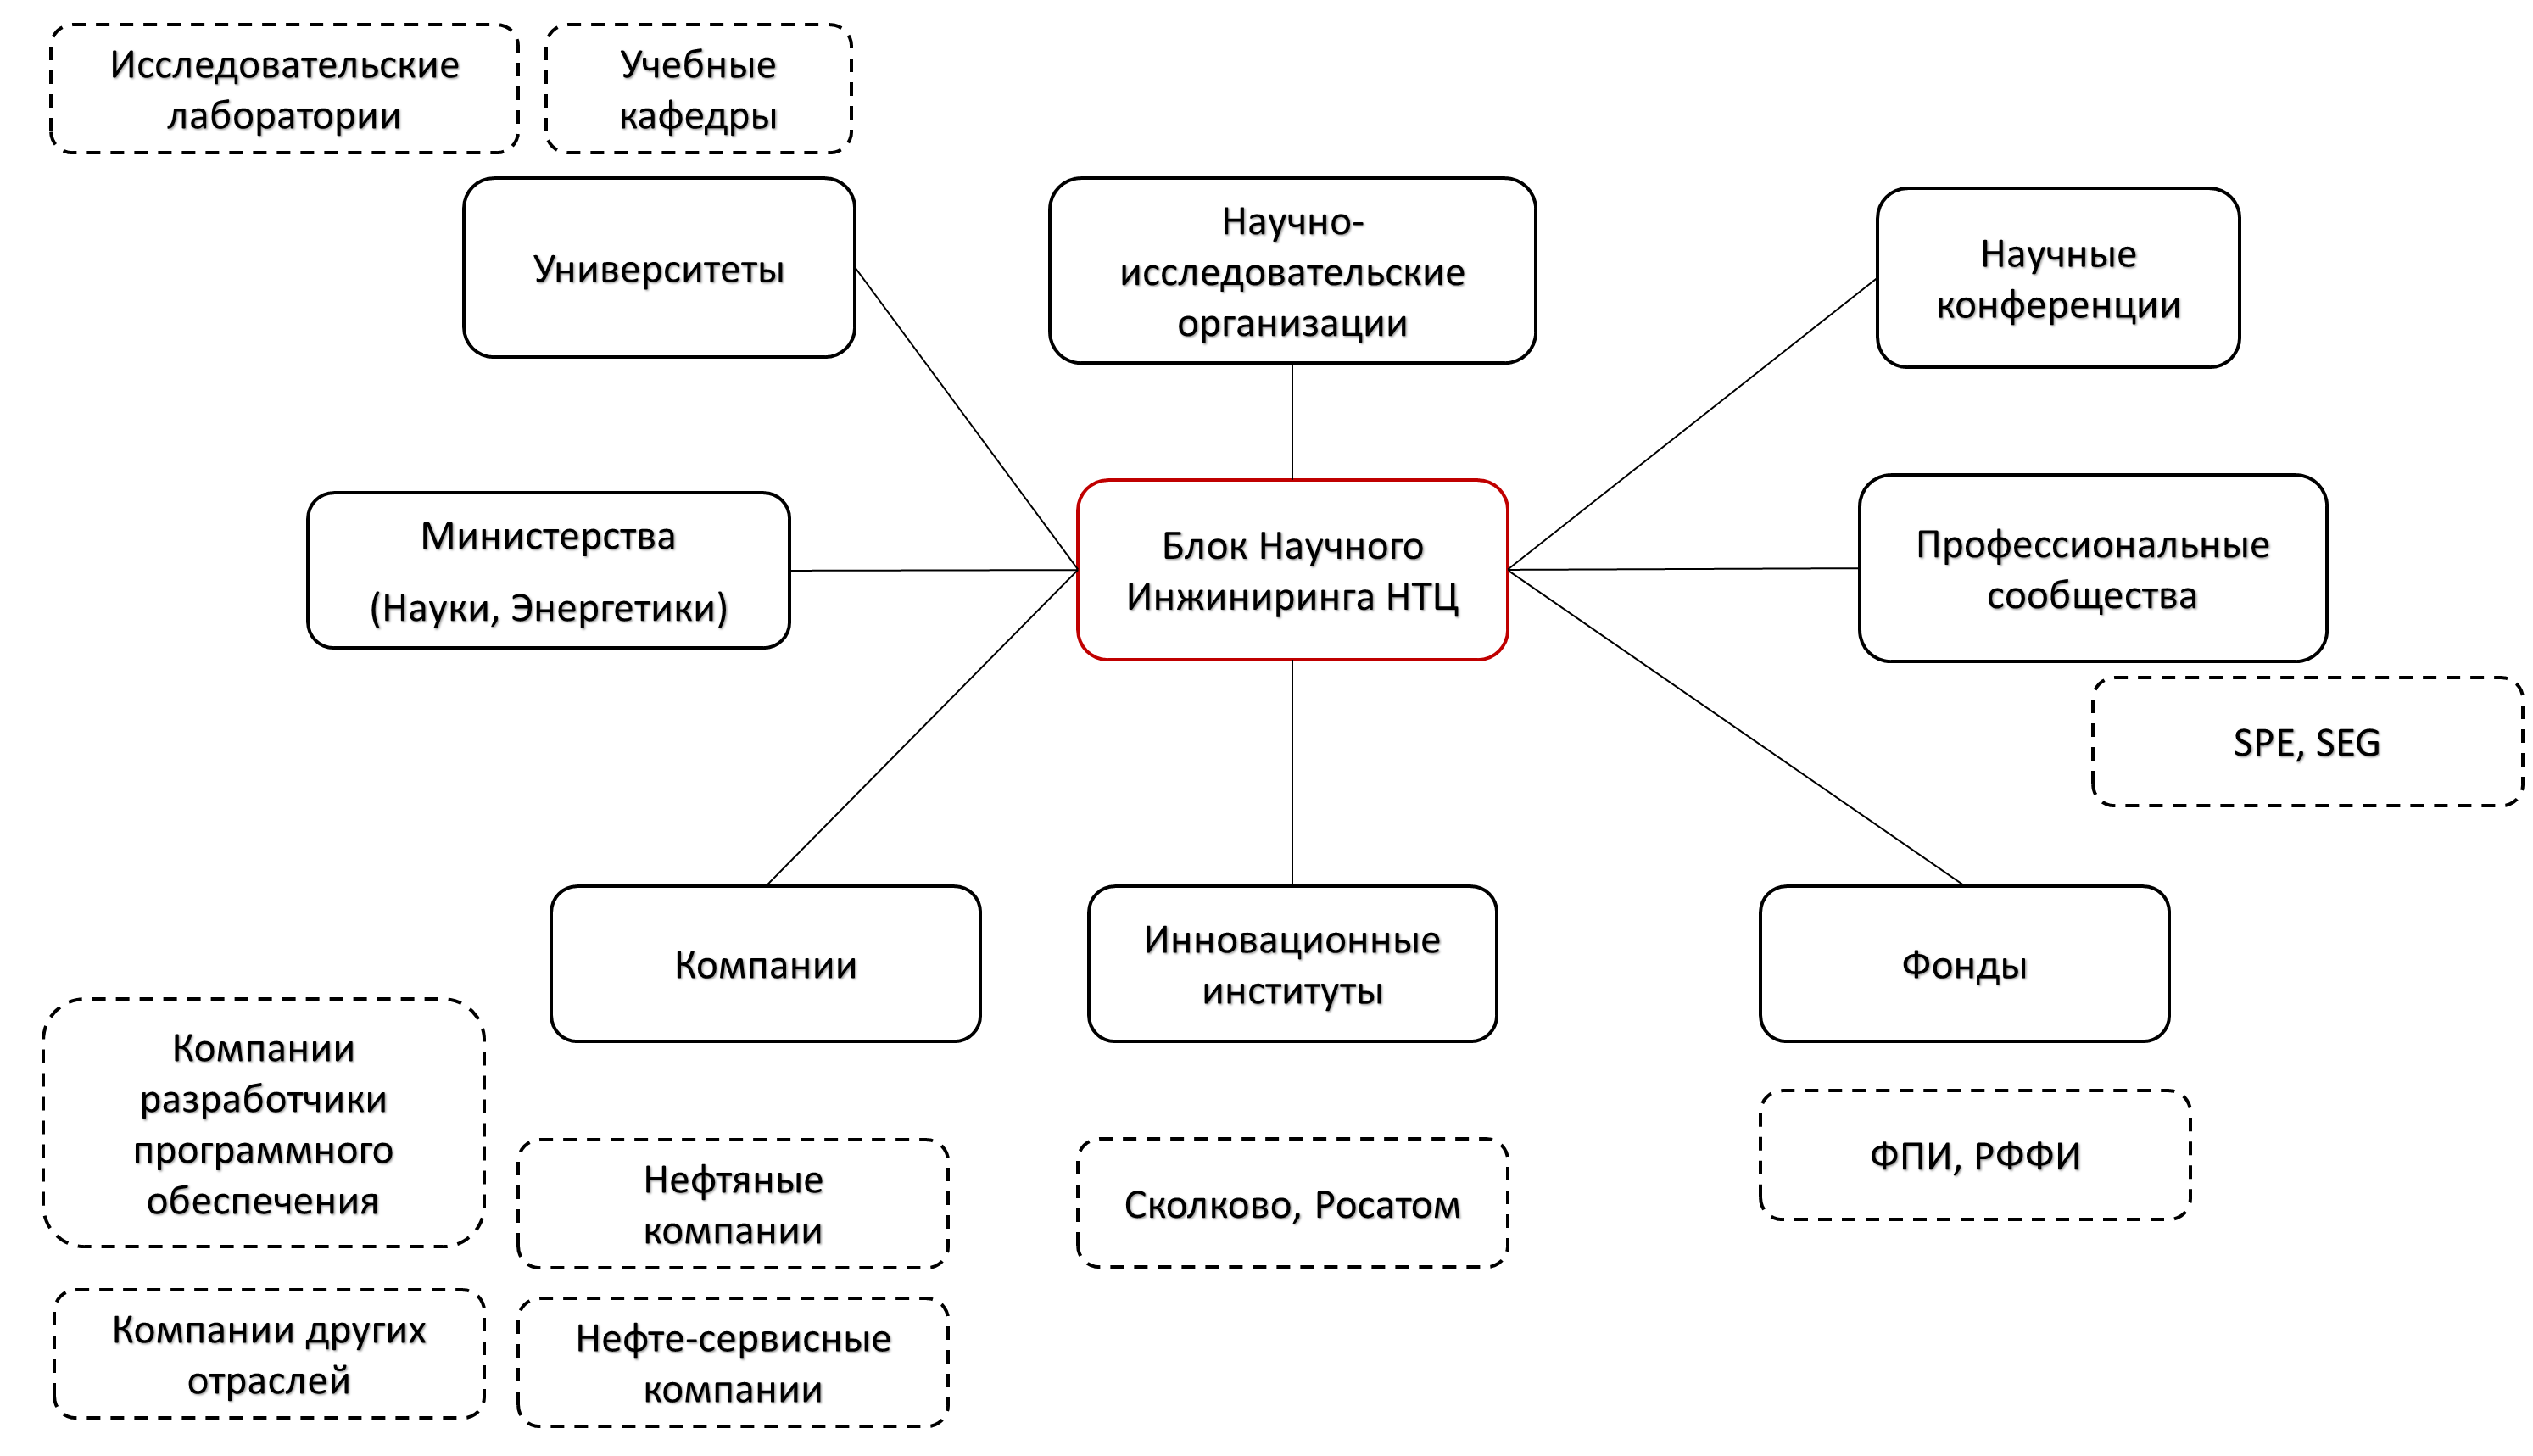
\includegraphics[width=\textwidth]{media/eco.png}
		%\caption{\label{fig:bim2} Спрос на услуги НТЦ.}
	\end{figure}
\end{frame}


\begin{frame}{Рынок услуг НТЦ}
\begin{figure}
	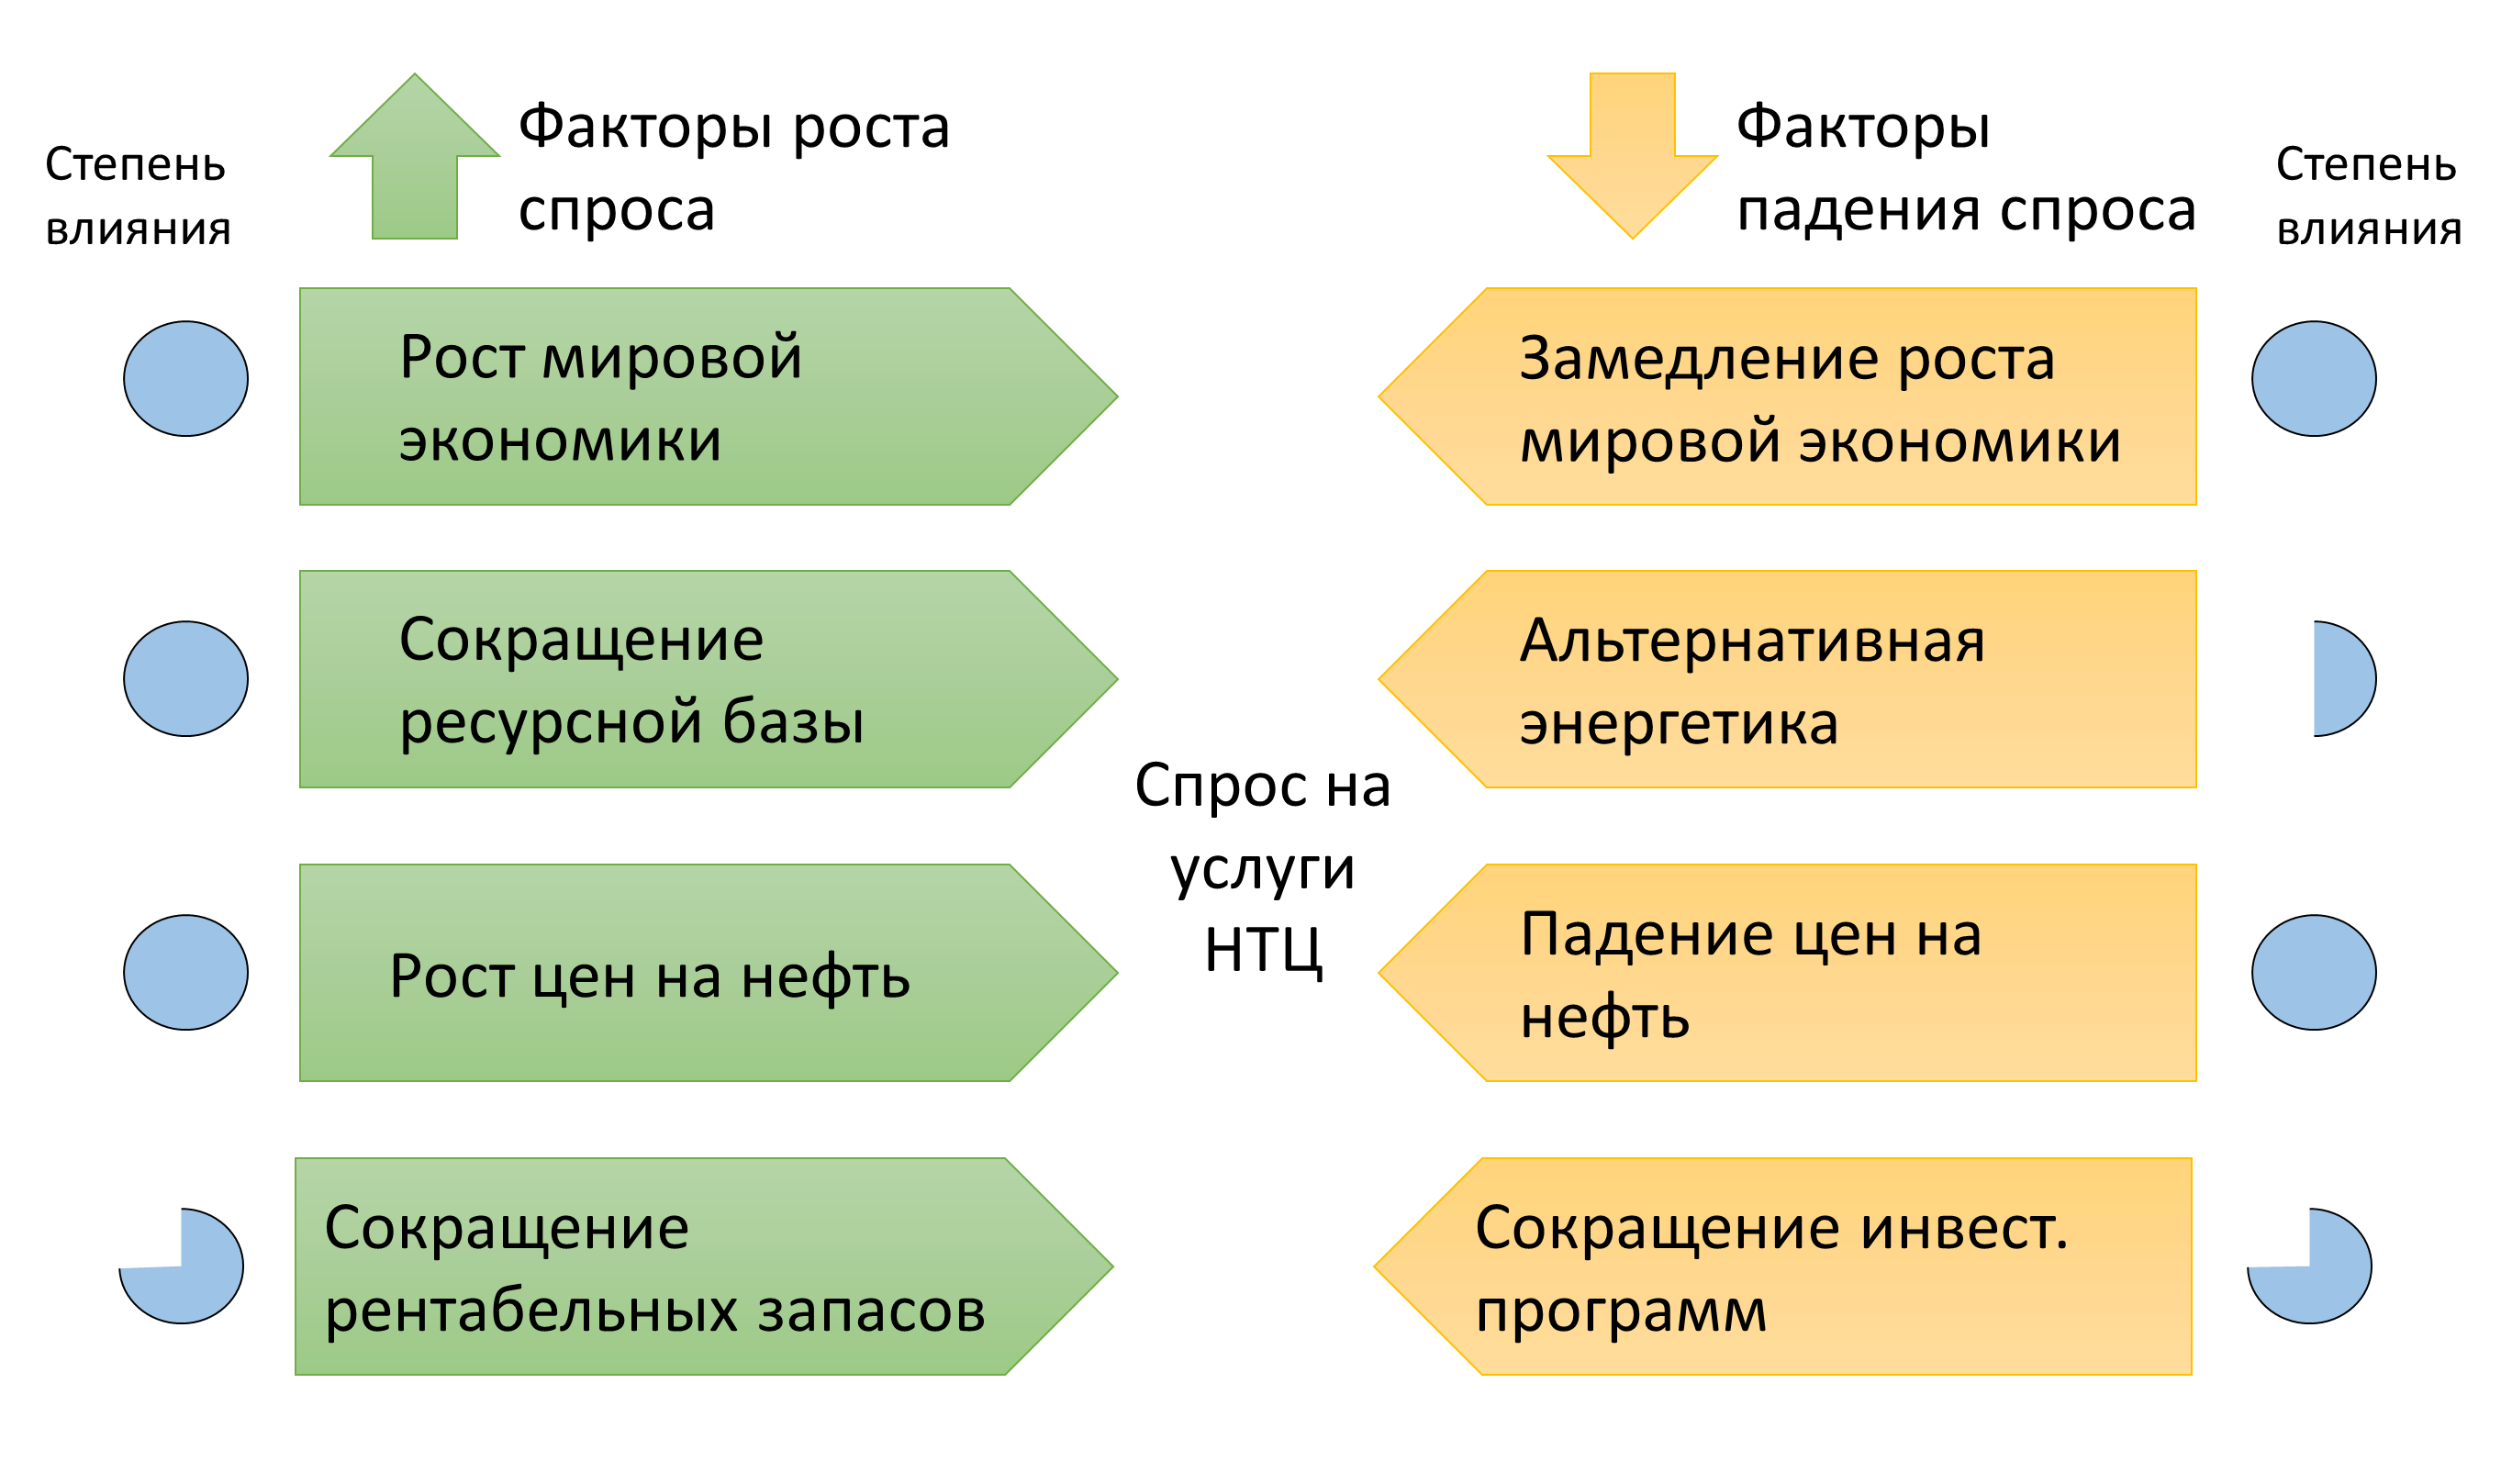
\includegraphics[width=\textwidth]{media/sANDd.png}
	%\caption{\label{fig:bim2} Спрос на услуги НТЦ.}
\end{figure}
\end{frame}


\begin{frame}{Цифровые двойники}
	\begin{figure}
		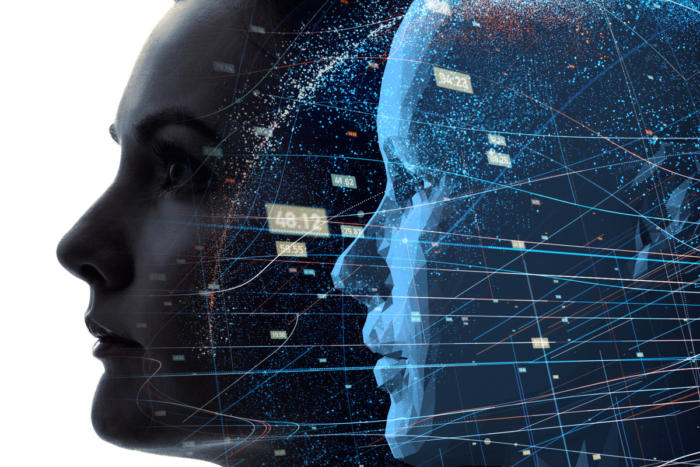
\includegraphics[width=\textwidth]{media/digital-twins_woman-in-profile_ai_mirror_duplicate_duo_pair-100760562-large.jpg}
	\end{figure}
	
	\tiny https://www.networkworld.com/article/3280225/what-is-digital-twin-technology-and-why-it-matters.html 
	
\end{frame}


\begin{frame}{Методический каркас исследования}
	\begin{figure}
		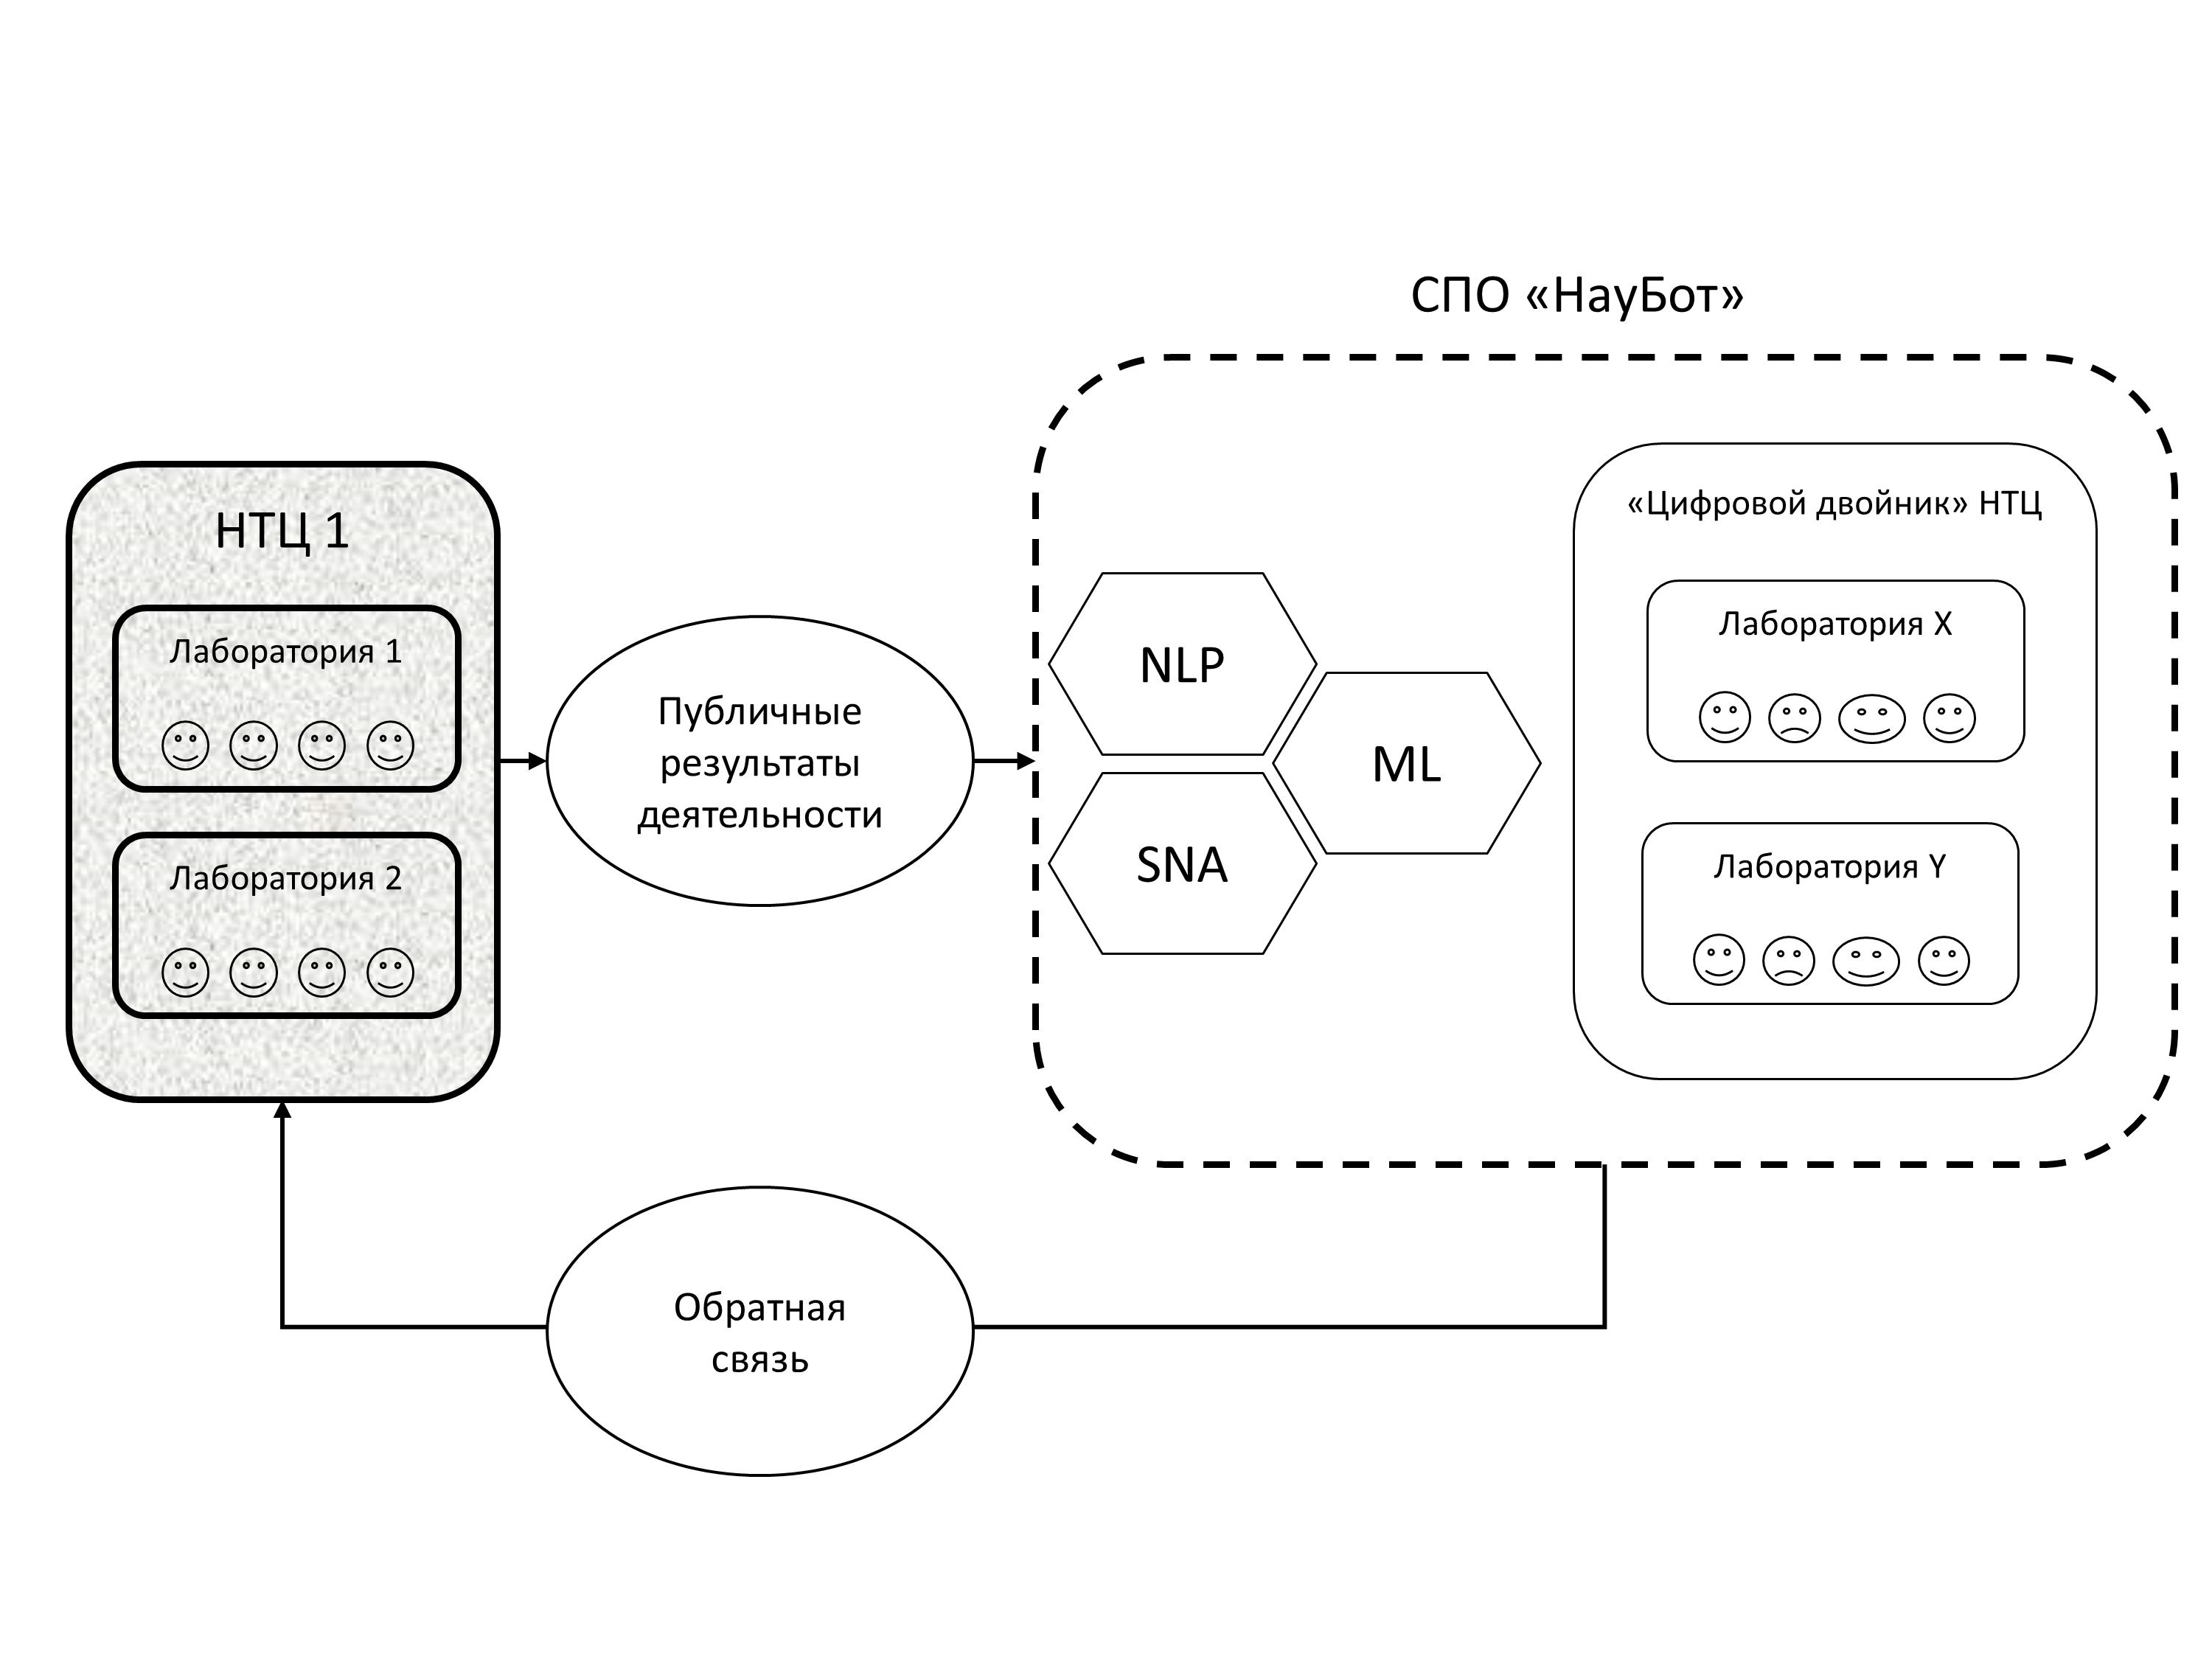
\includegraphics[width=\textwidth]{media/bim2.png}
		%\caption{\label{fig:bim2} Архитектура СПО``НауБот''.}
	\end{figure}
	
\end{frame}

\section{Цели исследования.}

\begin{frame}{Цели работы}
\begin{enumerate}
	\item Комплексный анализ, диагностика и моделирование социальных процессов в организационной среде;
	\item Поиск путей решения проблем обратной связи при прогнозировании путей развития НИР по определенным приоритетным направлениям;
	\item Разработка методов сбора и анализа результатов деятельности НТЦ для создания и обучения модели эффективности НТЦ с использованием алгоритмов машинного обучения и практик работы с "большими данными";
	\item Построение прогнозов о результатах деятельности НТЦ.
\end{enumerate}
\end{frame}

\begin{frame}{Постановка эксперимента для прямой и обратной задач.}
	
	\begin{itemize}
		\item \textit{Изучение деятельности НТЦ по внешним проявлениям.} \\
		К внешним проявлениям относятся цифровые артефакты деятельности организации - это опубликованные научные статьи, материалы конференций, информационные сайты в сети Интернет и новости о компании;
		\item \textit{Изучение НТЦ изнутри.} \\
		К исследованиям в этом направлении относятся моделирование научной деятельности, эффективность производственных процессов, самоорганизации малых творческих коллективов и модели персонала научной организации.
	\end{itemize}
\end{frame}

\section{Методы исследования.}

\subsection{Анализ социальных сетей.}
\begin{frame}{Социальная сеть: Граф соавторов.}
	\begin{figure}
		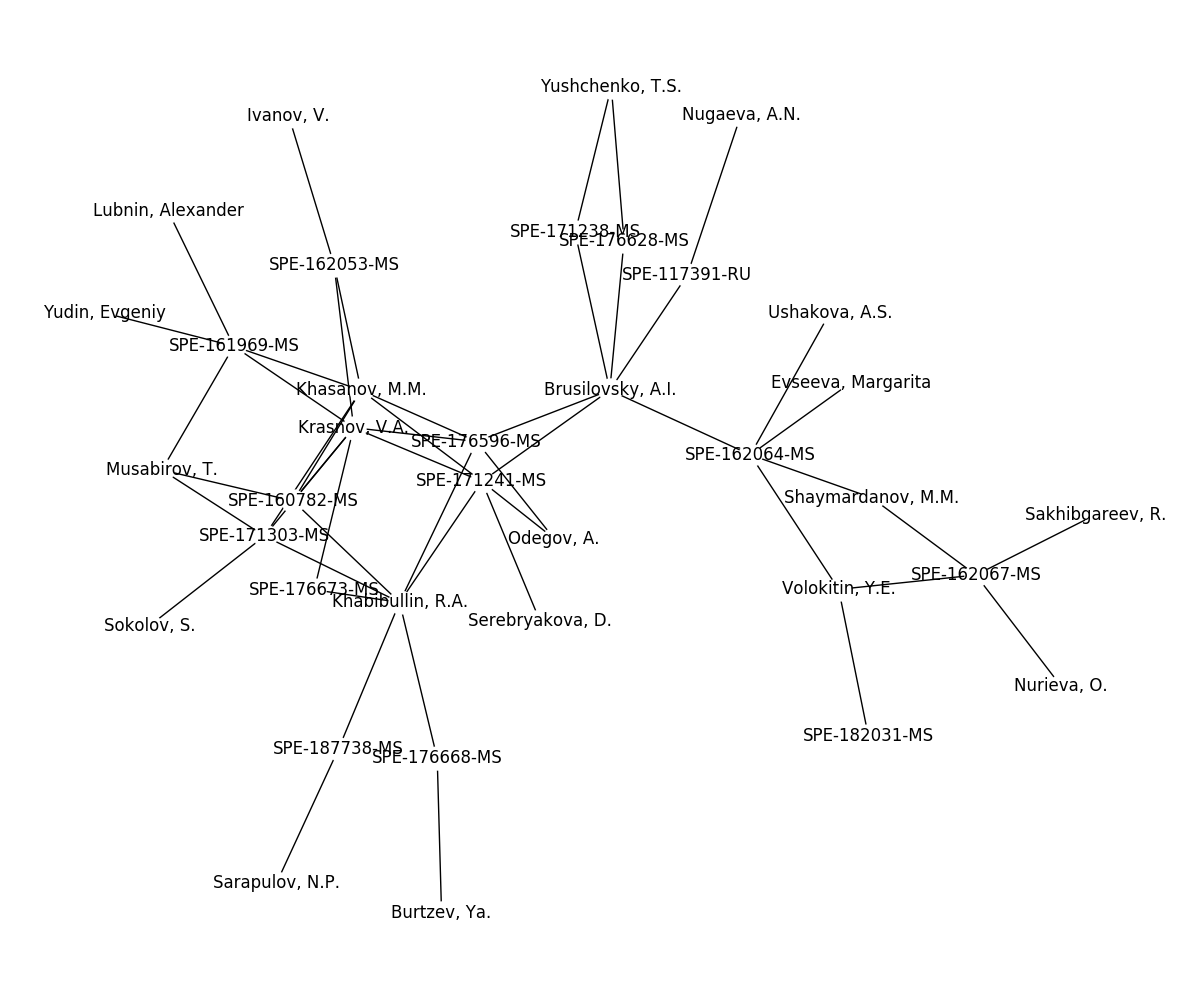
\includegraphics[width=0.9\textwidth]{media/allo6eng.png}
		%\caption{\label{fig:bim2} Архитектура СПО``НауБот''.}
	\end{figure}
\end{frame}

\begin{frame}{Социальная сеть: Метрики графа.}
	\begin{itemize}
		\item Для ребер
		\begin{itemize}
			\item Common Neighbours (CN)
			\item Salton Index (SI)
			\item Jaccard Index (JI)
			\item Hub Promoted Index (HPI)
			\item Hub Depressed Index (HDI)
			\item Leicht-Holme-Newman Index (LHN1)
			\item Preferential Attachment Index (PA)
			\item Adamic-Adar Index (AA)
			\item Resource Allocation Index (RA)
		\end{itemize}
		\item Для вершин 
		\begin{itemize}
			\item Degree centrality
			\item Betweenness centrality
			\item Closeness centrality
			\item Harmonic centrality
			\item Clustering
		\end{itemize}
	\end{itemize}
\end{frame}

\subsection{Анализ естественного языка}
\begin{frame}{Анализ естественного языка (Natural Language Understanding)}
Допустим у нас есть вероятность последовательности из $n$ слов $ P(w_1, \dots, w_n)\mbox{ , }$ такая, что вероятность третьего слова $P(w_3) $ равна $P(w_3|w_1,w_2)$. 
Тогда следующее выражение определяет вероятностную модель текста. 
\begin{equation}
	P ( w ) = P( w_1, w_2, \dots , w_n ) =  \prod_i^n P( w_i | w_1, w_2, \dots , w_{i-1} )
\end{equation}
Так как вычисление $P (w) $ представляет сложность $O^n$, то современные исследования текста используют представление $P ( w )$, как однородной Цепи Маркова и строят приближенные модели: 

\begin{itemize}
	\item Униграмная модель $ P(w_1, w_2, \dots , w_n )  \approx \prod_i^n P(w_i)$
	\item Биграмная модель $ P(w_i \vert w_1, w_2, \dots , w_{i-1} )  \approx  \prod_i^n  P(w_i \vert w_{i-1} )$
\end{itemize}

\end{frame}

\subsection{Многоагентное моделирование}
\begin{frame}{Многоагентное моделирование}
	\begin{figure}[ht]
		\centering
		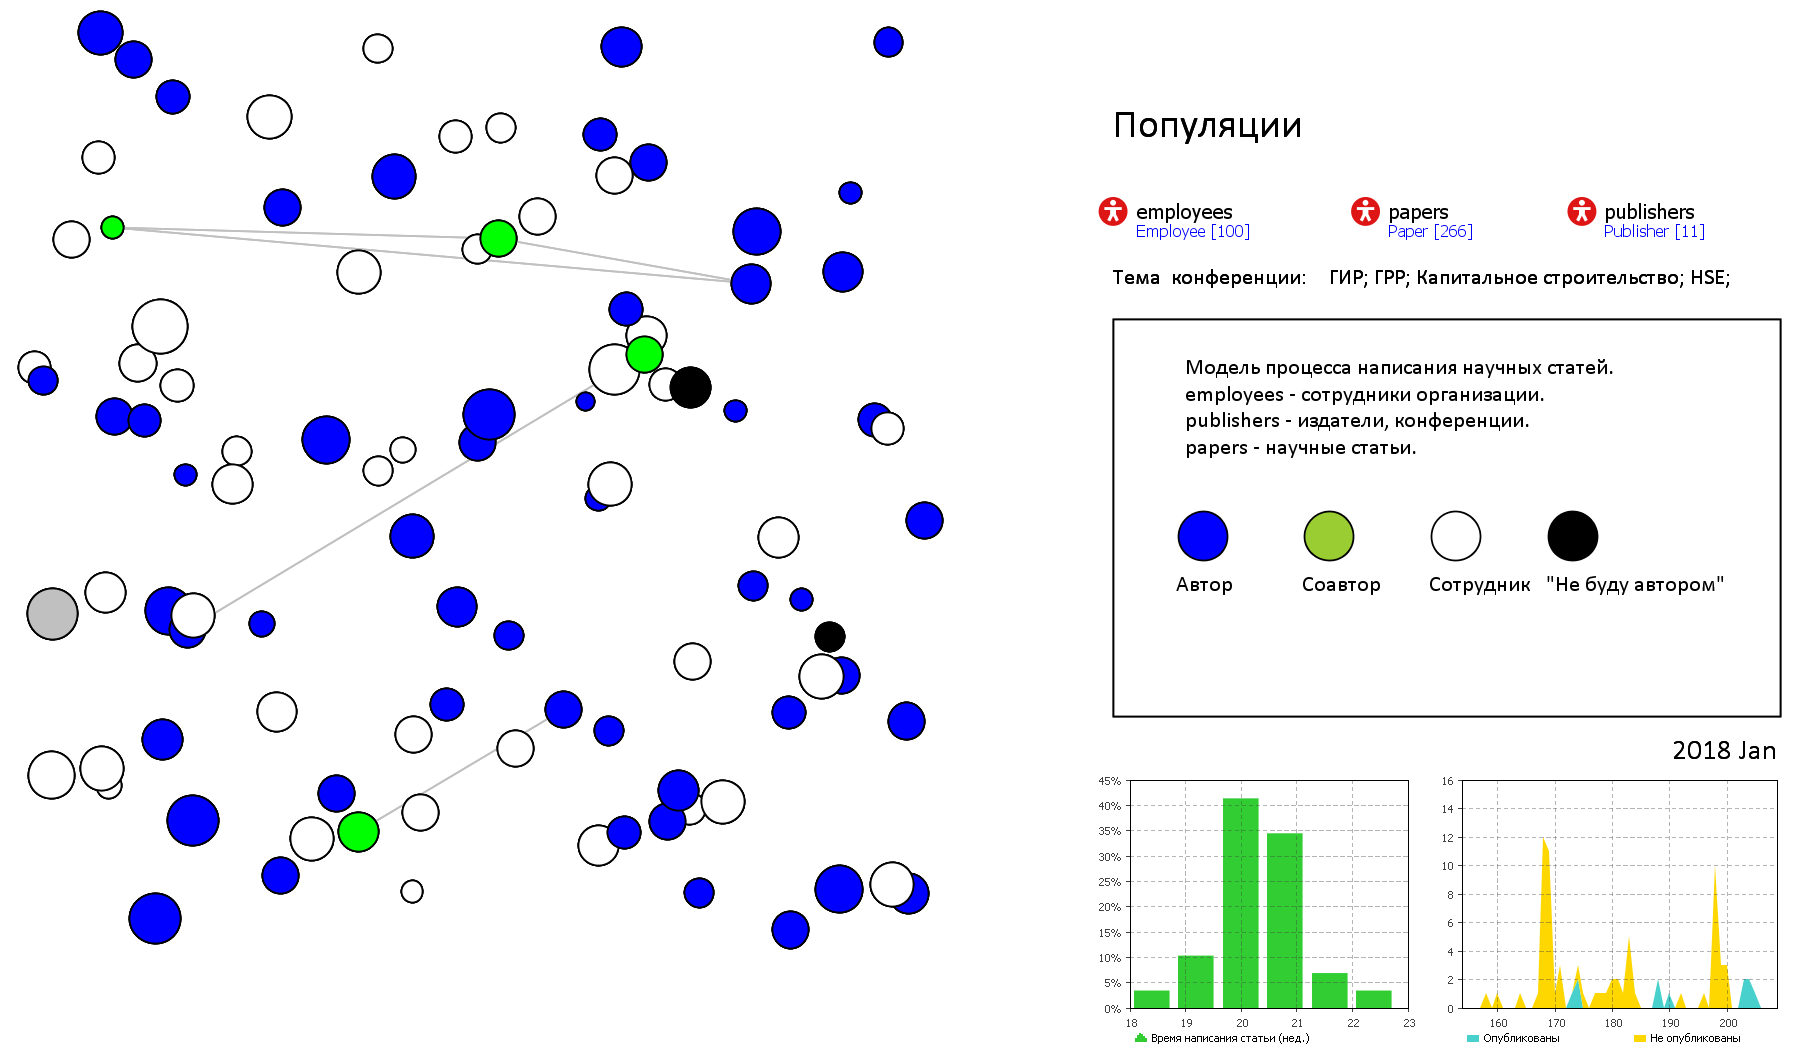
\includegraphics[width=0.9\textwidth]{media/so1}
		%		\caption{The cognitive map of the task model.}%
		%		\label{fig:icmon2}
	\end{figure}  
\end{frame}

\section{Научная новизна}

%\begin{frame}{Байесовские методы для определения параметров НТЦ}
%	Пусть дана функция $ \Psi \left(  x \right)$  и нам нужно найти $x$ при котором она достигает максимума $ \Psi   \left(  x \right) \longrightarrow \max_x$. Добавим условие, при котором расчет каждого значения $ \Psi   \left(  x \right)$ -- это ресурсоемкая задача. Такое условие встречается в следующих случаях: 
%	
%	\begin{itemize}
%		\item $x$ - это географические координаты скважины, а $ \Psi   \left(  x \right)$ - это количество нефти, которое можно добыть, пробурив скважину с координатами $x$. В таком случае одно значение $ \Psi   \left(  x \right)$ стоит миллионы рублей;
%		\item $x$ - это гиперпараметры искусственной нейронной сети глубокого обучения, $ \Psi   \left(  x \right)$  - это целевая метрика точности предсказания. В этом случае одно значение $ \Phi   \left(  x \right)$ будет занимать месяцы работы;
%	\end{itemize}
%\end{frame}
%

%\begin{frame}{EM-алгоритм с регуляризацией (I)}
%%	Научный текст является одним из проявлений деятельности НТЦ. %
%%	Выявление тематик текста может быть сделано с использованием распределения Дирихле. 
%	Байесовская модель для постериорного распределения скрытых тематик в тексте может быть записана в следующем виде.
%	\begin{eqnarray*} \label{eq:lda1}
%		p \left( W,\Phi,\Theta \right) = \prod_{d=1}^{D} p \left( \theta_d \right) \prod_{n=1}^{N_d} p \left( \phi_{dn} \vert \theta_d \right) p \left( w_{dn} \vert \phi_{dn} \right) \\
%		p \left( \theta_d \right) \sim Dir(\alpha) \\
%		p \left( \phi_{dn} \vert \theta_d \right) = \theta_{d\phi_{dn}} \\
%		p \left( w_{dn} \vert \phi_{dn} \right) = \Phi_{\phi_{dn}w_{dn}} \\
%		\sum_w \Phi_{tw} = 1 \\
%		\Phi_{tw} \geqslant 0
%	\end{eqnarray*}
%	Таким образом, что $W$ - это текстовые данные ,  $\Phi$ - распределение слов в каждой тематике, $\Phi$ - распределение тематик для каждого слова, $\Theta$ - распределение тематик в документе.
%\end{frame}

%\begin{frame}{EM-алгоритм с регуляризацией}
%
%	Оптимизационная задача для поиска скрытых тематик выглядит следующим образом: 
%	\begin{equation} \label{eq:lda2}
%	P(W \vert \Phi) \rightarrow max_\Phi
%	\end{equation}
%	
%	Для использования ЕМ-алгоритма выпишем явно уравнения для Е-шага и М-шага:
%	
%	\textbf{Е-шаг:}
%	\begin{equation}\label{eq:lda3}
%	\mathcal{KL} (q(\Theta) \, q(\Phi) \vert \vert p \left( \Theta,\Phi \vert W \right) ) + \mu * R(q(\Theta) \, q(\Phi)) \rightarrow \underset{q(\Theta) \, q(\Phi)} {\text{minimize}}
%	\end{equation}
%	
%	\textbf{М-шаг:}
%	\begin{equation}\label{eq:lda4}
%	\mathbb{E}_{q(\Theta) \, q(\Phi)} \log p \left( \Theta,\Phi,W \right) \rightarrow \underset{\Phi}{\text{maximize}}
%	\end{equation}
%\end{frame}

\begin{frame}{Моделирование научных направлений}
\begin{itemize}
	\item \textbf{Гипотеза о существовании научных направлений:}\\
	Каждое вхождение термина $w$  в научную статью $d$ связано с научным направлением $t$ из заданного множества $T$.
	\item \textbf{Гипотеза об условной независимости научных направлений:}\\
	Появление терминов $w$  в документе $d$ по научному направлению $t$ не зависит от документа $d$, а зависит только от $t$ и может быть описано единым распределением $p(w | t) =  p(w | d,t) $
	\item \textbf{Оптимизационная задача:} 
	\begin{align}
	&\mathcal{L} (D,\Phi,\Theta)  \rightarrow \underset{\Phi \, \Theta}{\text{maximize}}& \quad &\\
	&\sum_{w \in W} \phi_{wt} = 1 &  \sum_{t \in T} \theta_{td} = 1 & \\
	& \phi_{wt} \geq 0 & \theta_{td}  \geq 0 & 
	\end{align}
\end{itemize}

\end{frame}

\begin{frame}{Двухшаговая оптимизация невыпуклой функции при моделировании научных направлений}	
	\begin{align*}
		&\textbf{Expectation step:}  \\  		
		& p_{tdw} \equiv  p(t|d,w) = \frac{p(w|t) p(t|d)}{p(w|d)} = \frac{\phi_{wt} \theta_{td}}{\sum_{\hat{t} \in T}\phi_{w {\hat{t}}} \theta_{\hat{t} d}} \\
	\end{align*}
	\begin{align*}
		&\textbf{Maximization step:}   \\
		& \phi_{wt} = \frac{n_{wt}}{\sum_{\hat{w} \in D}n_{\hat{w}t}}  & n_{wt} = \sum_{d \in D} n_{dwt} = \sum_{d \in D} n_{dw} p(t|d,w) \\		
		& \theta_{td} = \frac{n_{td}}{\sum_{\hat{t} \in T} n_{\hat{t}d}}  & n_{td}  = \sum_{w \in d} n_{dwt} = \sum_{w \in d} n_{dw} p(t|d,w)  \\		
	\end{align*}
\end{frame}

\begin{frame}{Стратегии регуляризации для выделения научных направлений}
	\begin{align*}
		\mathcal{KL} (q(\Theta) \, q(\Phi) \vert \vert p \left( \Theta,\Phi \vert D \right) ) + \sum_i \mu_i * R_i(q(\Theta) \, q(\Phi)) \rightarrow \underset{q(\Theta) \, q(\Phi)} {\text{minimize}}				
	\end{align*}
	\begin{itemize}
	\item Сглаживание $R = \alpha \sum_{w,t} \ln \phi_{wt}, R= \alpha \sum_{t,d} \ln \theta_{td}$ ;
	\item Разреживание $R = - \alpha \sum_{w,t} \ln \phi_{wt}, R= - \alpha \sum_{t ,d} \ln \theta_{td}$;
	\item Декорреляция $ R = \sum_{w \ne u, t} \phi_{wt} \phi_{ut}$;
	\item Увеличение когерентности $R = \sum_{w \ne u, t} C_{uw} (\phi_{wt}-\phi_{ut})^2$
	\item Лаплассиан графа документов $R = \sum_{\hat{t} \ne t, d} C_{\hat{t}t} (\theta_{\hat{t} d}-\theta_{td})^2$
	\end{itemize}
\end{frame}

%\subsection{Имитационное моделирование}

\begin{frame}{Имитационное моделирование}
	Допустим, что в отраслевой научно-исследовательской организации $\Omega$  работают лаборатории $\lambda_i$ , где $i \in (1 \dots N_{\lambda})$ . 
	Обозначим множество лабораторий $ \Lambda = \{ \lambda_i, \dots , \lambda_{N_{\Lambda}} \}$.
	В лабораториях работают научные сотрудники $ A = \{ a_{i}, \dots, a_{N_A} \} $. Обозначим множество научных направлений $t_i$, где $i \in (1, \dots, N_T )$, по которым организация $\Omega$ ведет НИР как $T = \{ t_1, \dots , t_{N_T} \}$. Тогда деятельность организации $\Omega$ по выполнению НИР может быть описана следующими компонентами :
	\begin{equation} 
	\label{eq:so1}
	\mathbb{M}_{\Omega} = \bigg \{ S, \Xi, \Psi, E \bigg \} \mbox {, где }  S = \{ \Lambda, A, T, P, X \}
	\end{equation} 
	
	\begin{itemize}
		\item $ \Xi = \{ \xi_1 , \dots , \xi_{N_{\Xi}} \} $ -- множество связей между субъектами,
		\item $ \Psi = \{ \psi_1 , \dots , \psi_{N_{\Psi}} \} $ -- множество действий субъектов,
		\item $ P = \{ \rho_1 , \dots , \rho_{N_P} \} $ -- множество научных работ,
		\item $ X = \{ \chi_1 , \dots , \chi_{N_X}  \} $ -- множество научных журналов и конференций.
	\end{itemize}
	
\end{frame}

\section{Результаты эксперимента}

\begin{frame}{Модель образования малых команд}
	\begin{figure}
		\centering
		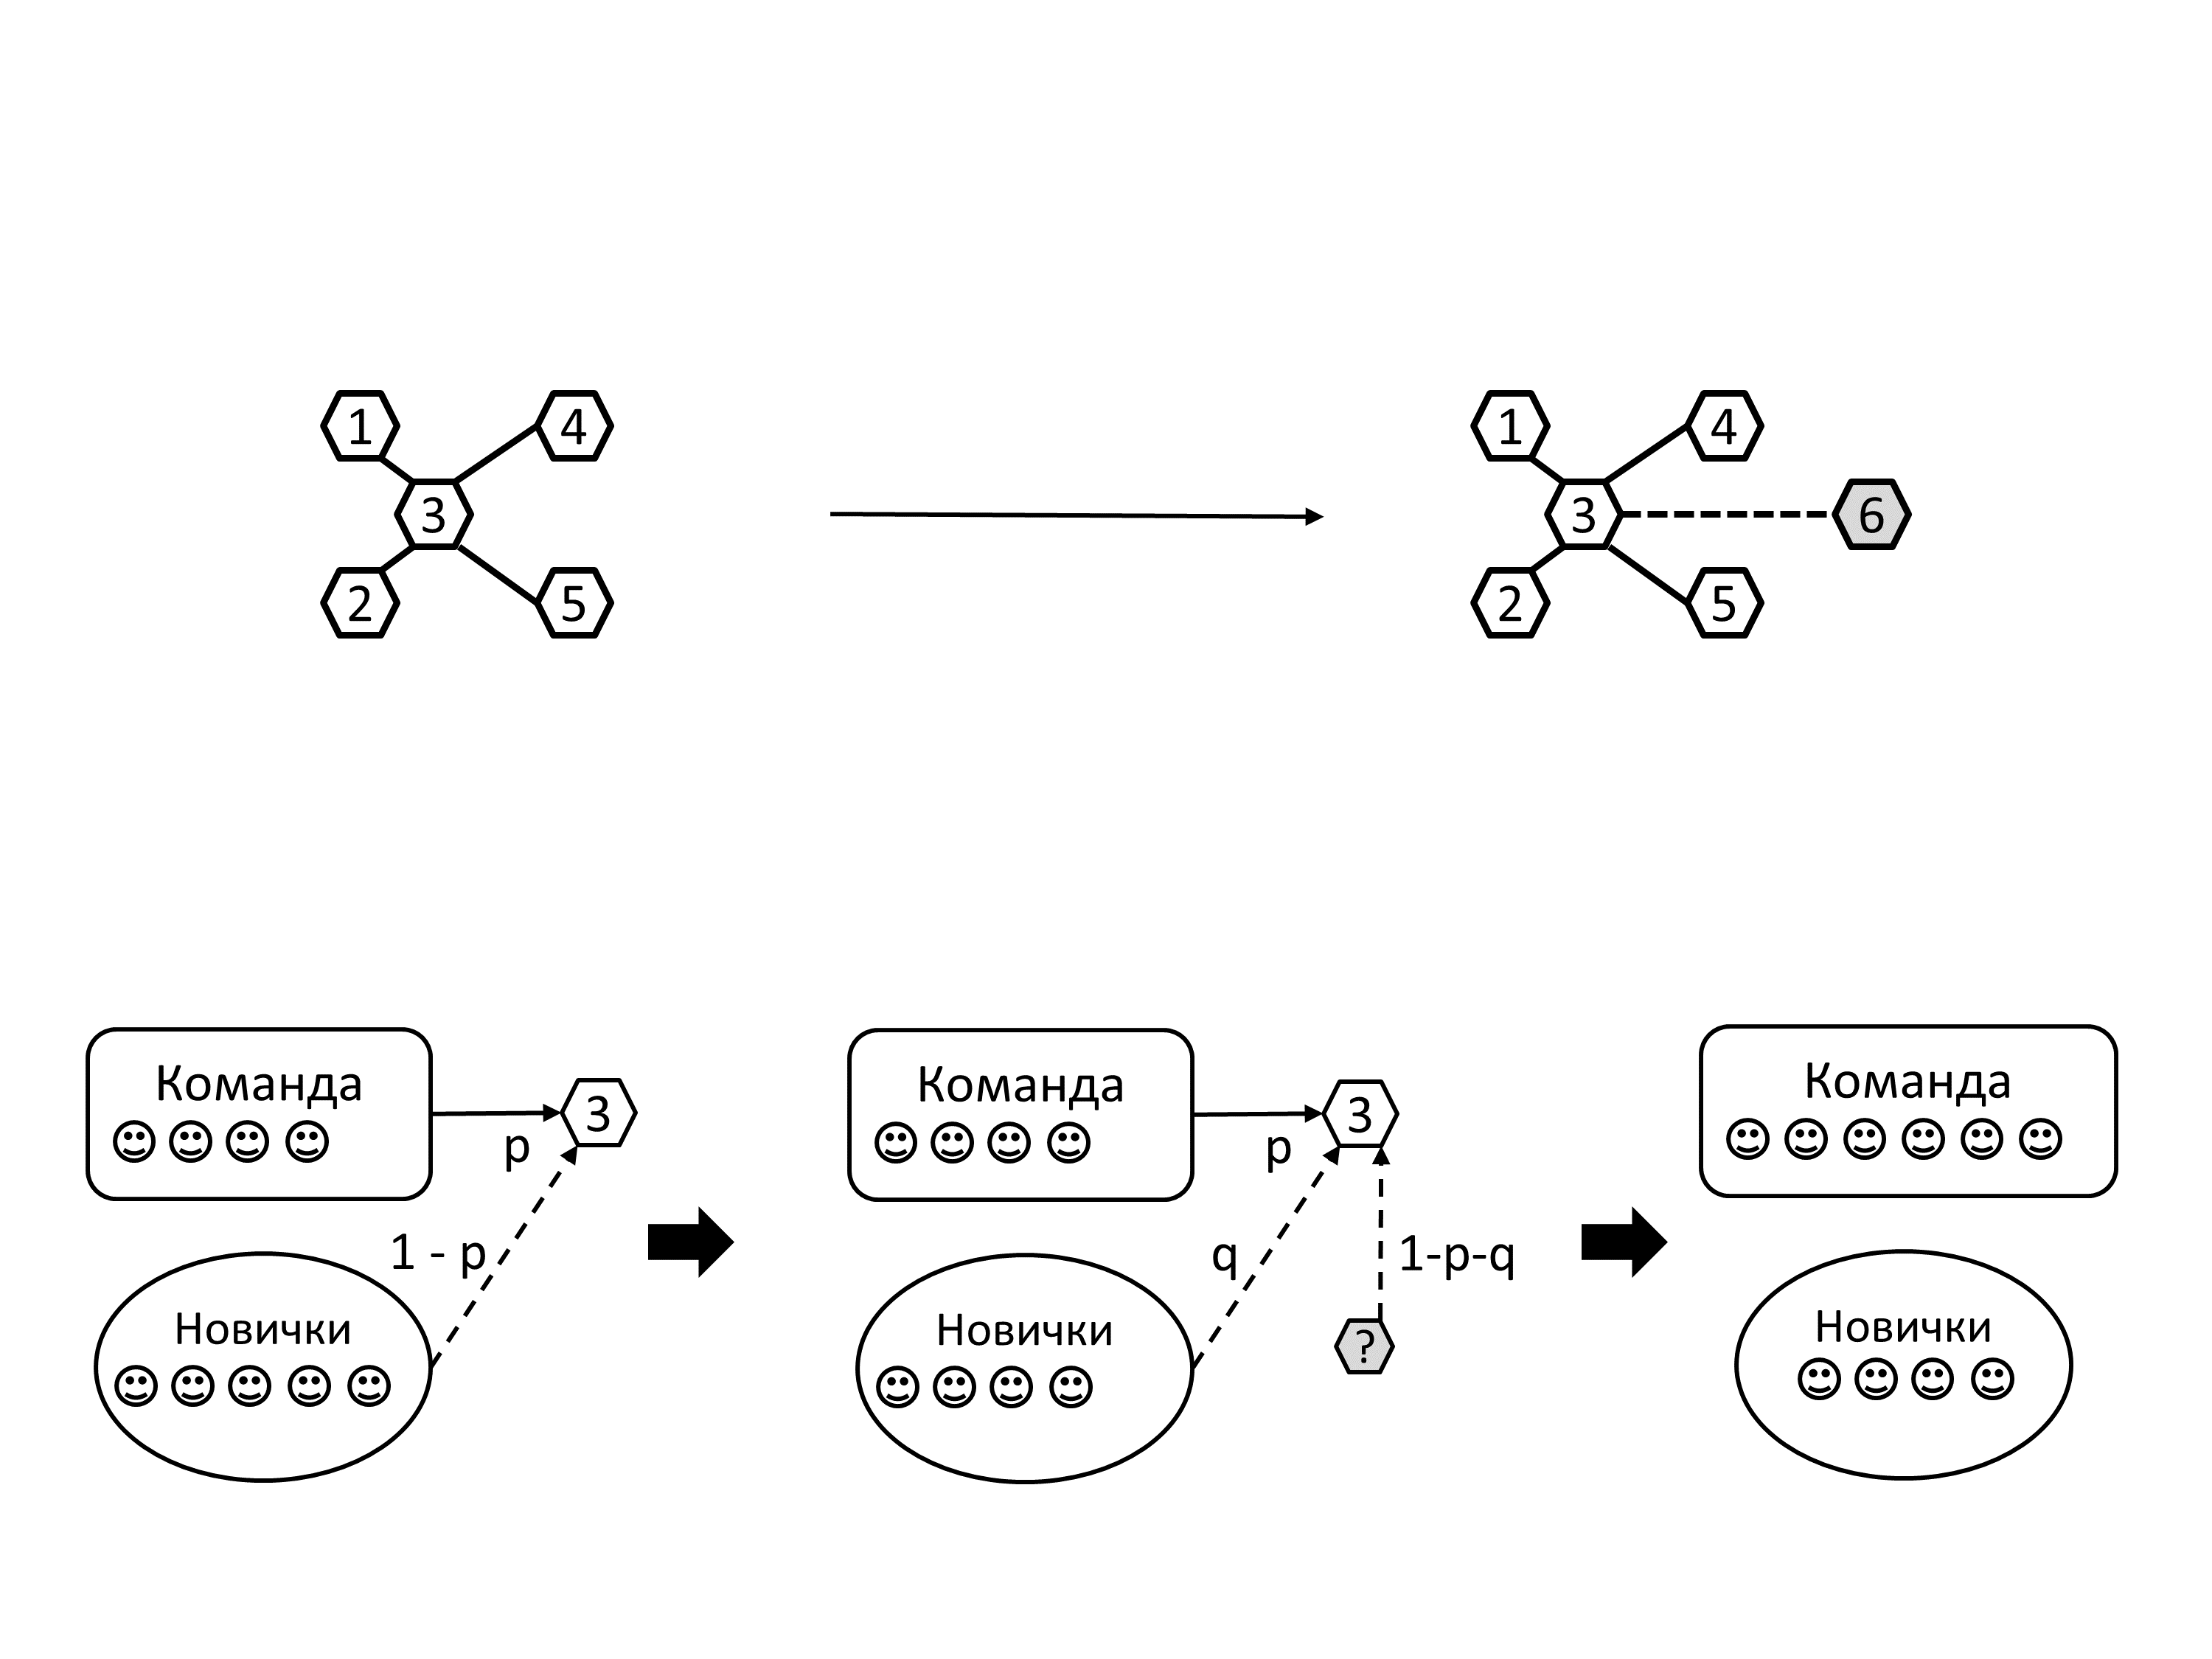
\includegraphics[width=0.9\textwidth]{media/bim3.png}
		%\caption{\label{fig:bim2} Архитектура СПО``НауБот''.}
	\end{figure}
\end{frame}

\subsection{Модель персонала}
\begin{frame}{Модель персонала}
	\begin{figure}[ht]
		\centering
		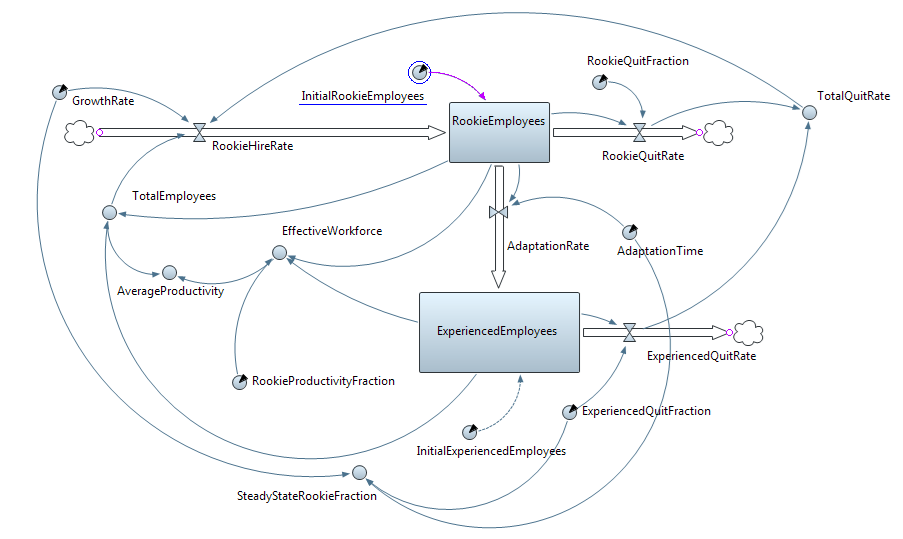
\includegraphics[width=0.9\textwidth]{media/icmon1}
		%		\caption{The cognitive map of the task model.}%
		%		\label{fig:icmon2}
	\end{figure}  
\end{frame}

\begin{frame}{Модель выполнения заданий}
	\begin{figure}[ht]
		\centering
		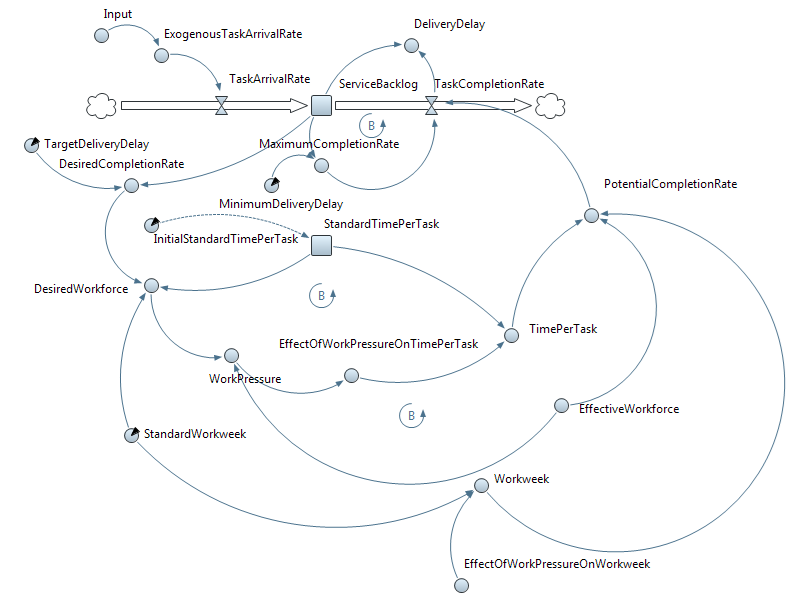
\includegraphics[width=0.8\textwidth]{media/icmon2}
%		\caption{The cognitive map of the task model.}%
%		\label{fig:icmon2}
	\end{figure}  
\end{frame}

\subsection{Модель проведения исследований}
\begin{frame}{Модель проведения исследований}
	\begin{figure}[ht]
		\centering
		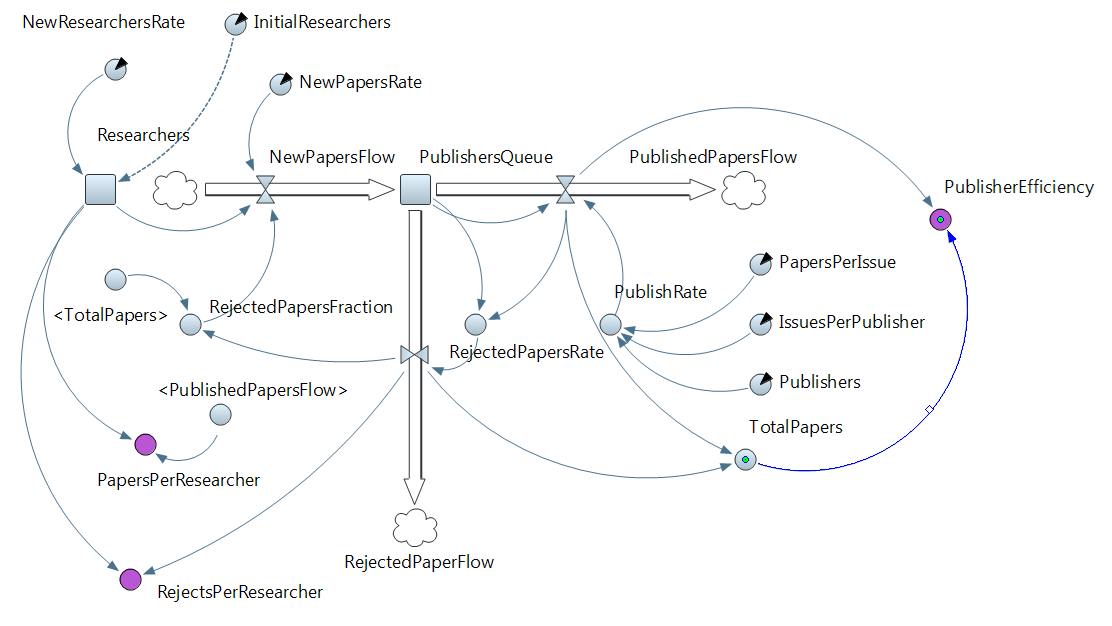
\includegraphics[width=0.9\textwidth]{media/om6}
		%		\caption{The cognitive map of the task model.}%
		%		\label{fig:icmon2}
	\end{figure}  
\end{frame}



\subsection{Синтетический граф соавторства}
\begin{frame}{Синтетический граф соавторства}
	\begin{figure}[ht]
		\centering
		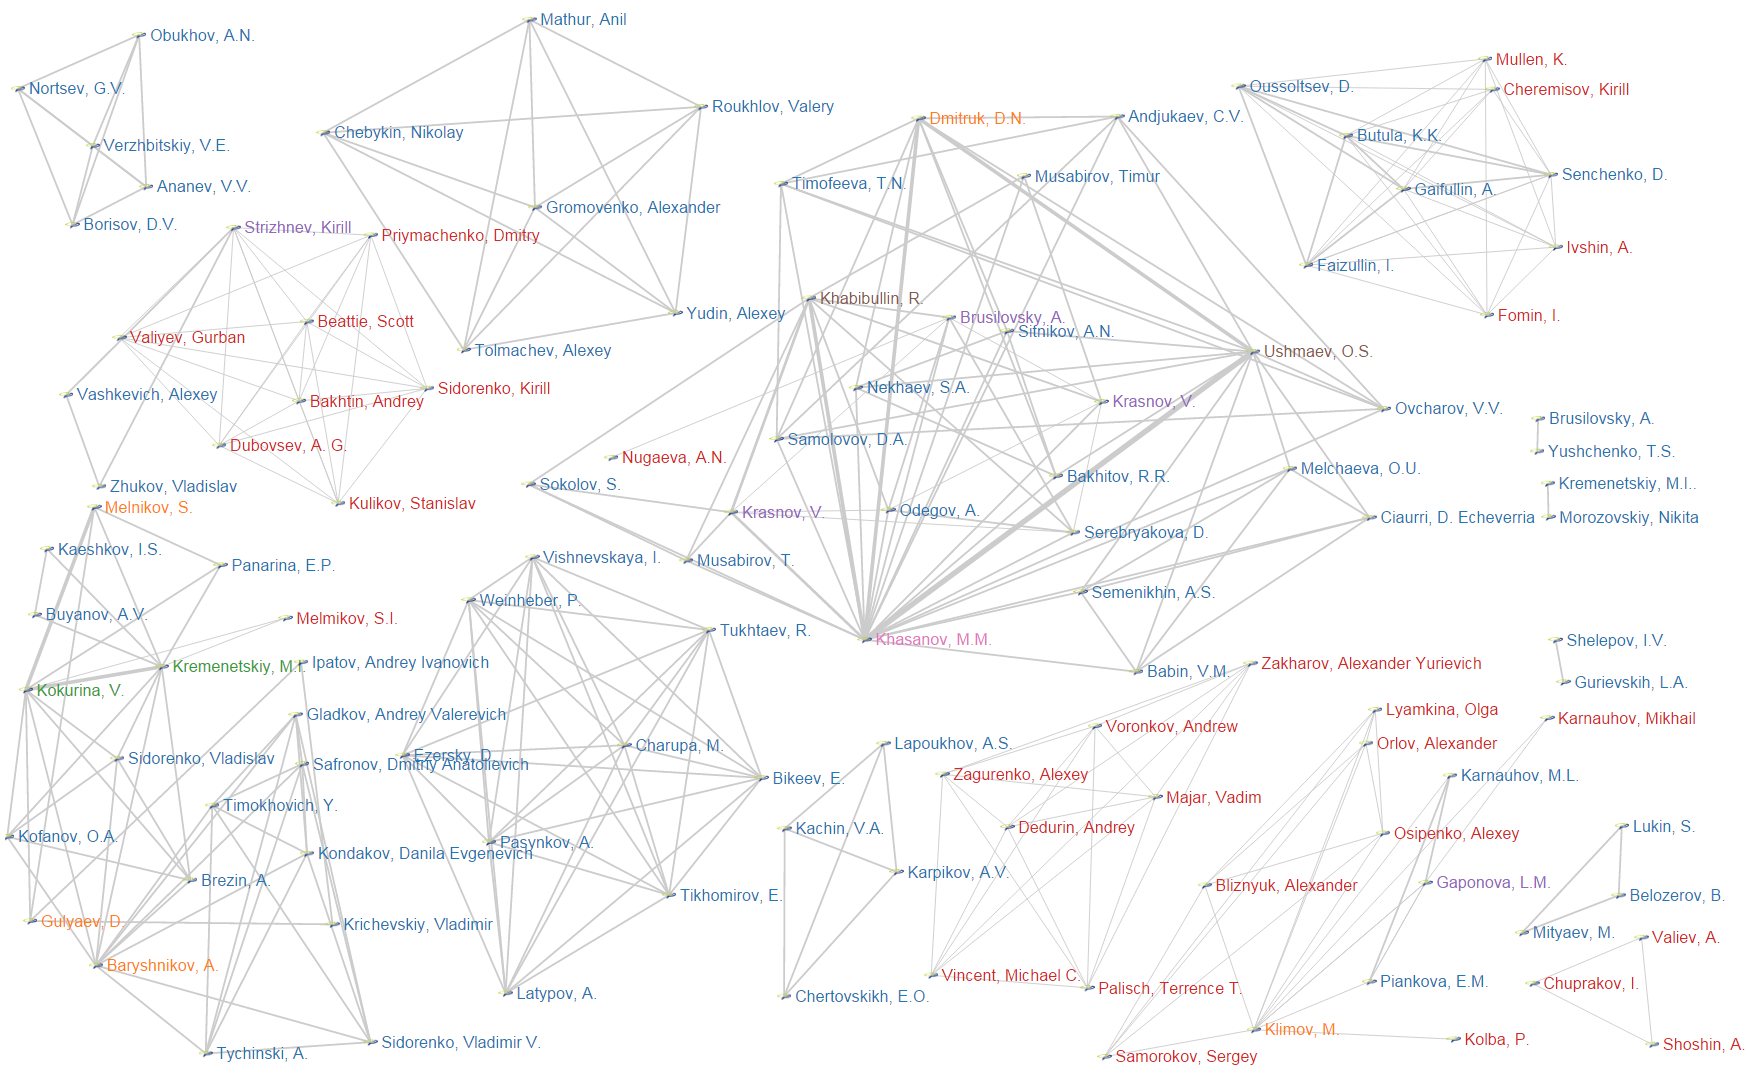
\includegraphics[width=0.9\textwidth]{media/so3}
		%		\caption{The cognitive map of the task model.}%
		%		\label{fig:icmon2}
	\end{figure}  
\end{frame}

\begin{frame}{Кластеризация графа соавторства на основе алгоритма "обратного распада".}
	\begin{figure}[!ht]
		\centering
		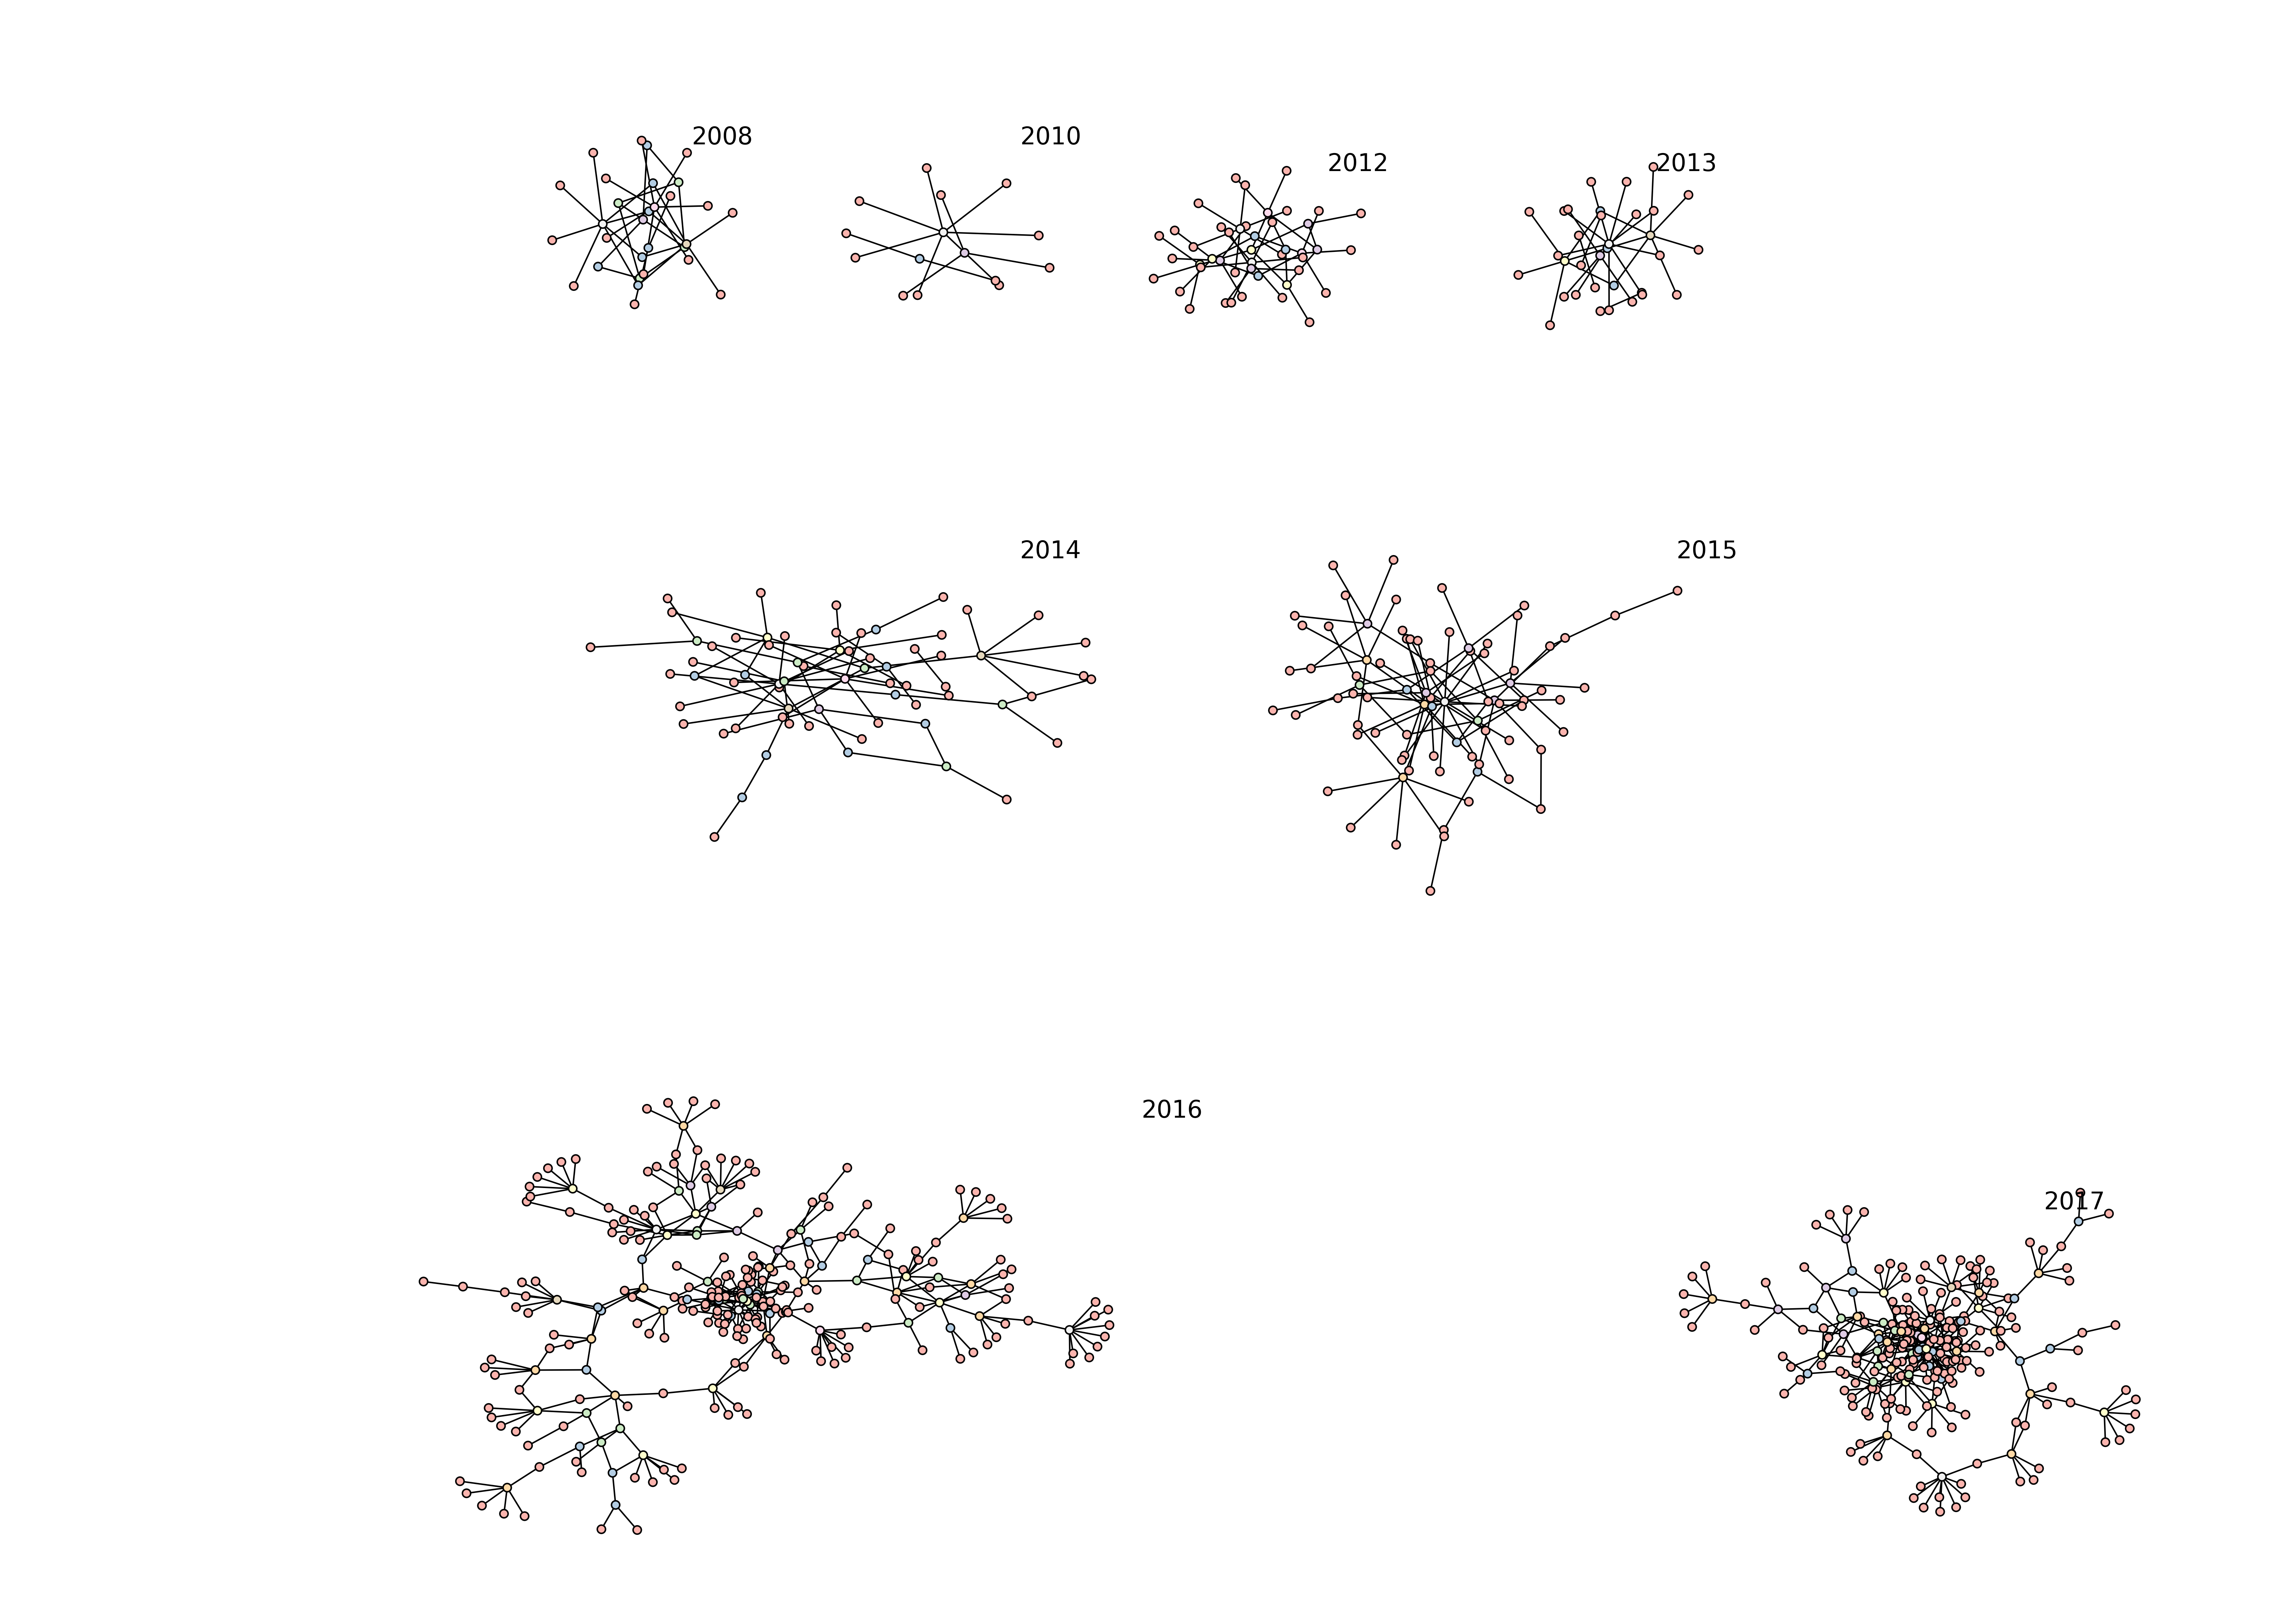
\includegraphics[width=0.95\textwidth]{media/guest3.png}
%		\caption{The co-authorship development growth dynamic by year graph.}
%		\label{fig:guest3}
	\end{figure}
\end{frame}


\begin{frame}{Сходимость численных методов вероятностного тематического моделирования}
	\begin{figure}
		\begin{center}
			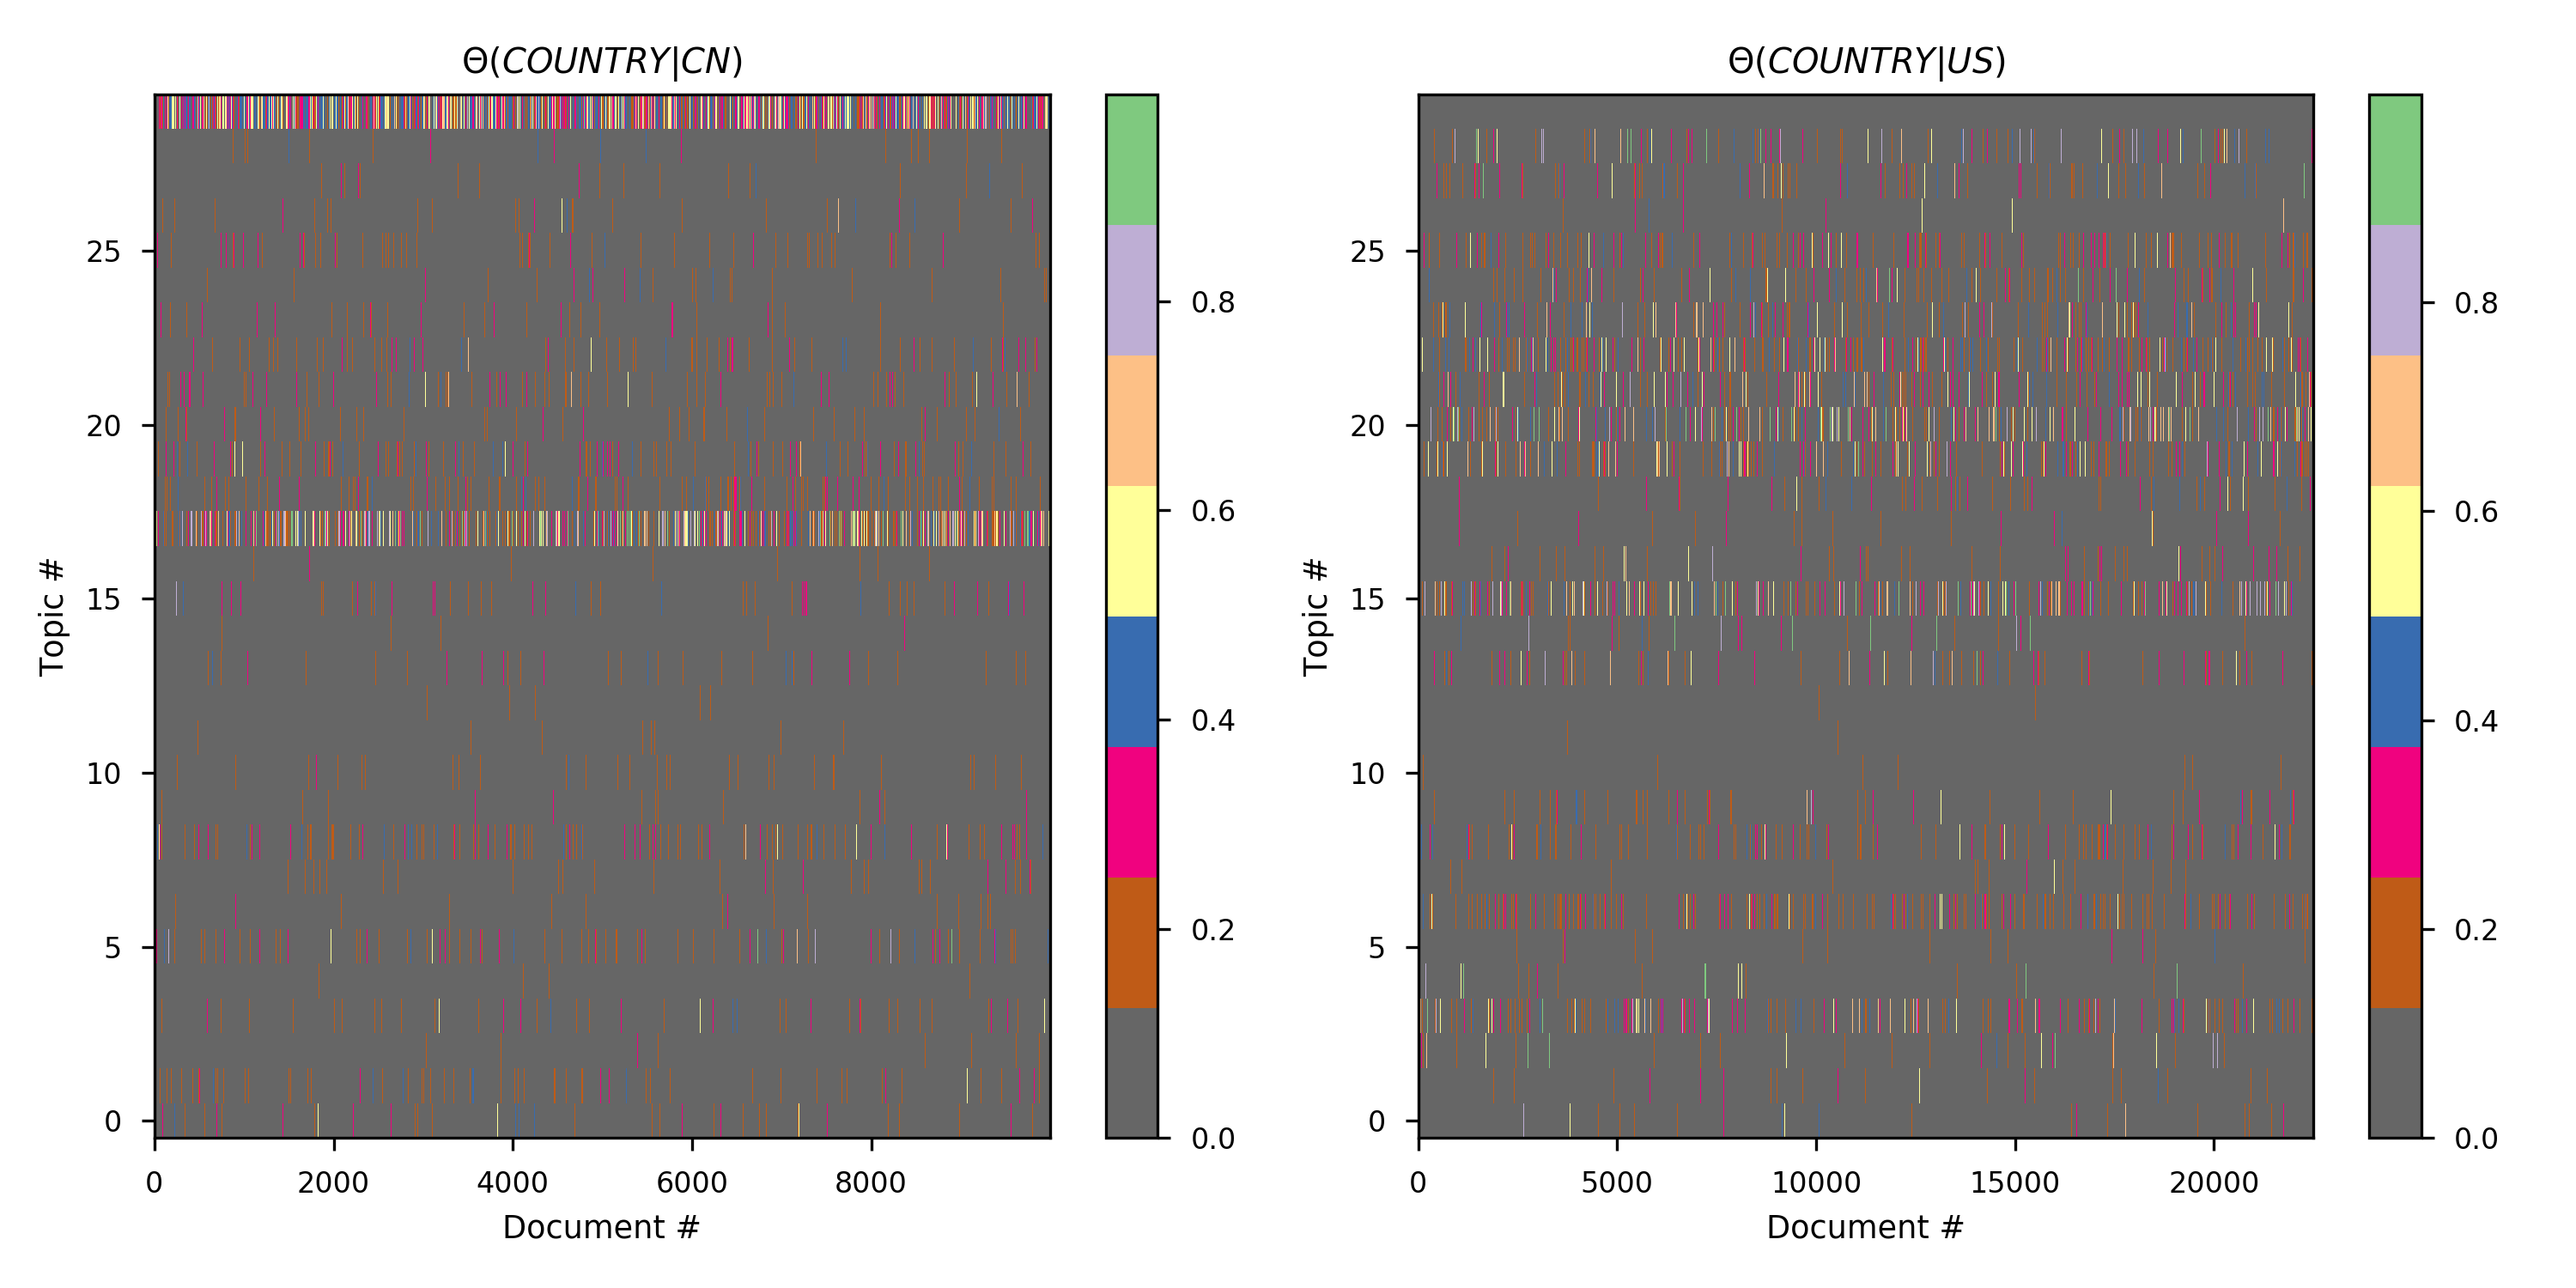
\includegraphics[width=0.95\textwidth]{media/op37fig3eng}
		\end{center}
	\end{figure}
	\begin{block}{}
		Автор разработал стратегию регуляризации для выделения научных направлений. 
	\end{block}
\end{frame}

\begin{frame}{Основной результат}
	Создана аппаратно-аналитическая платформа СПО ``НауБот'' для моделирования научной деятельности НТЦ на основе алгоритмов машинного обучения и имитационного моделирования. 
	\begin{figure}
		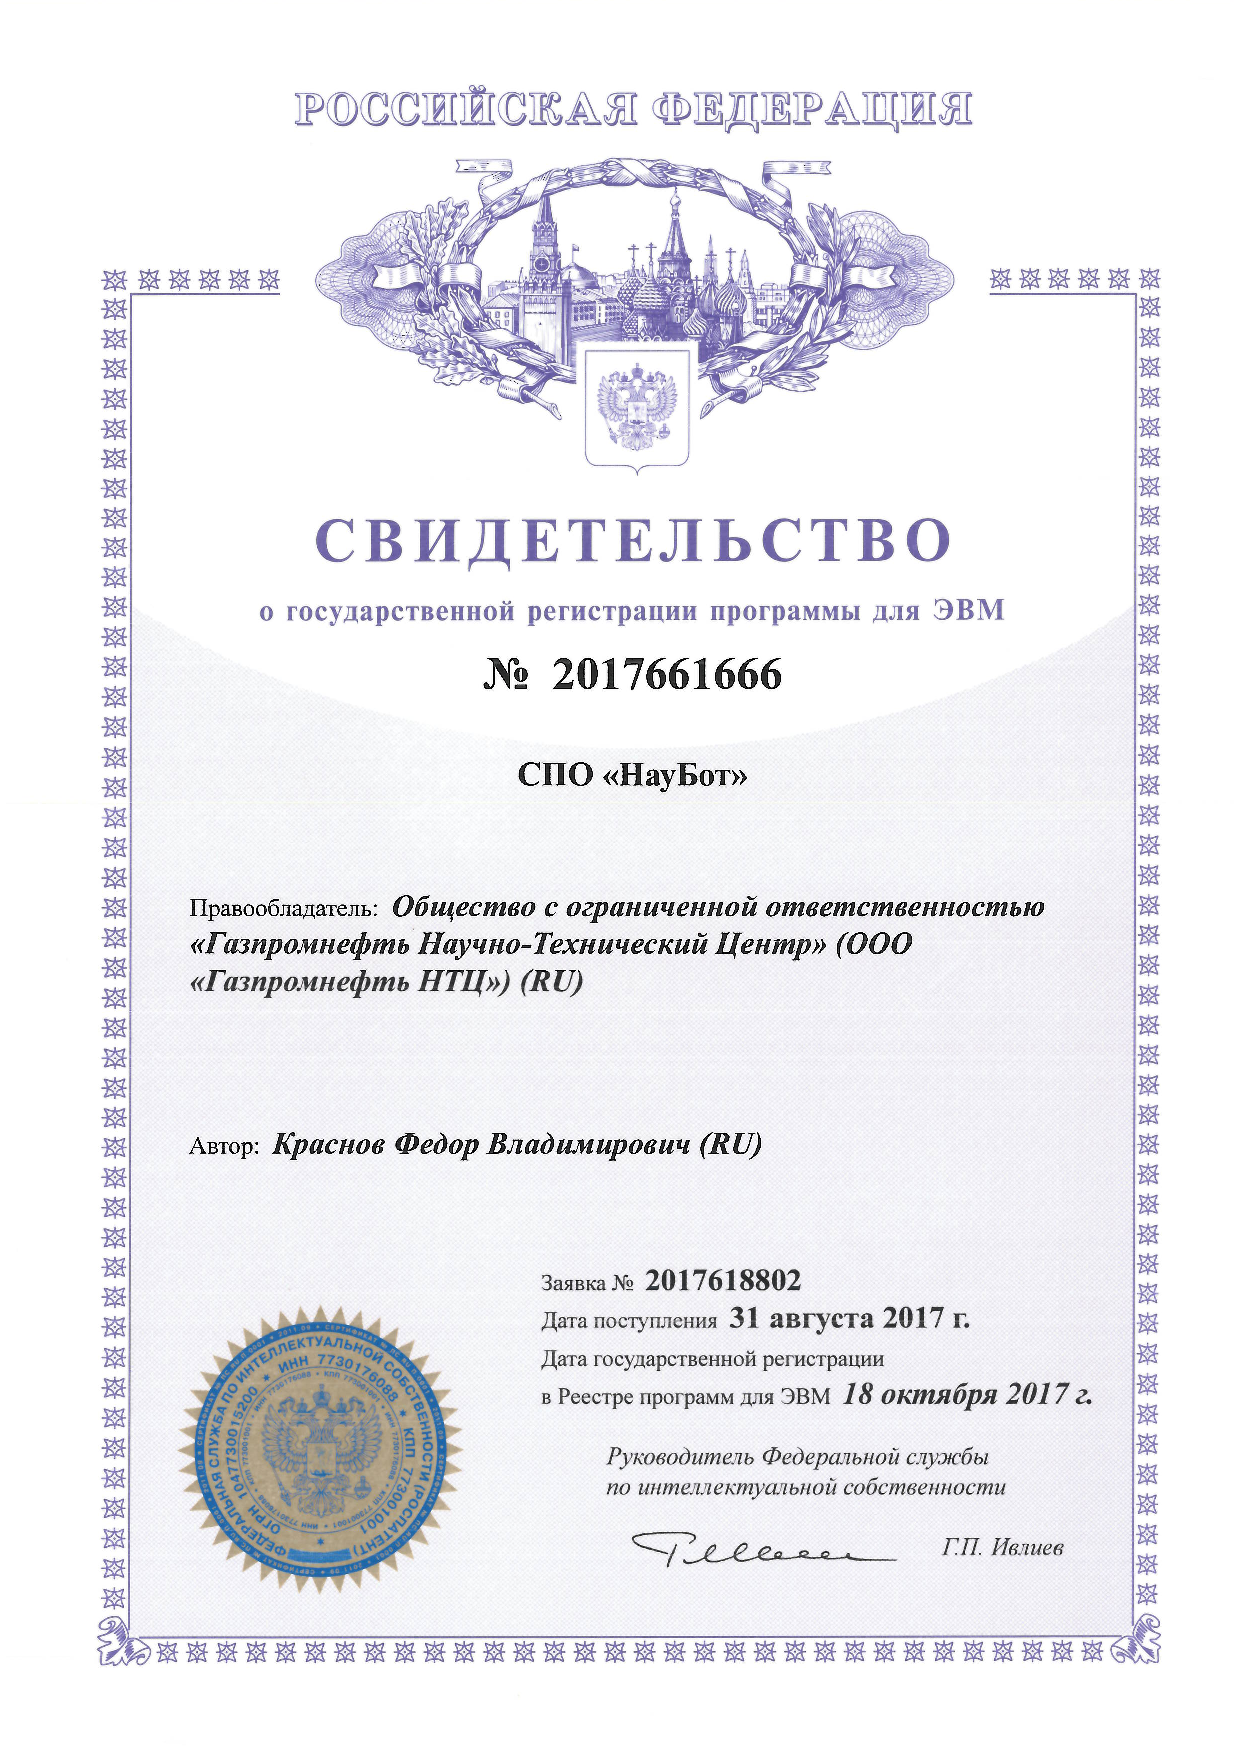
\includegraphics[width=0.4\textwidth]{media/naubot.pdf}
		\caption{\label{fig:naubot} Свидетельство регистрации программы для ЭВМ.}
	\end{figure}
	
\end{frame}


\begin{frame}{Результаты работы}
	\begin{enumerate}
		\item Предложена формализация процесса самоорганизации команд для достижения определённой цели;
		\item Разработан детальный алгоритм образования соавторств;
		\item Исследована временная зависимость структуры соавторств;
		\item Создана модель для прогнозирования соавторств;
		\item Создана модель научных направления развития НТЦ на основе публичных данных о публикационной активности сотрудников;
		\item Создана модель движения персонала в организации и модель выполнения наукоемких заданий;
		\item Разработан математический аппарат построения графов соавторства на основе двудольного графа;
		\item Построен ``цифровой двойник'' НТЦ.
	\end{enumerate}
\end{frame}


\begin{frame}{Практическая значимость результатов исследования}
	По теме исследования опубликовано более \textbf{40} работ; \textbf{20} из них опубликованы в рецензируемых научных изданиях, рекомендованных ВАК. 
	
	Доклады автора опубликованы в \textbf{6} сборниках из списка Web of Science. 
	
	Получены \textbf{3} свидетельства о регистрации программ для ЭВМ.
%	\begin{block}{title}
	\linebreak
	\linebreak
	Результаты, полученные в ходе настоящего исследования – модели, методы, алгоритмы, комплексы программ были использованы для решения практических задач по оценке научной эффективности НТЦ в энергетической отрасли.
%		Предлагаемые модели и методы могут быть распространены на НТЦ из других отраслей и на научно-исследовательские (НИ) организации при условии, что они представлены цифровыми артефактами научной деятельности.
%	\end{block}
\end{frame}

\end{document}
